\documentclass[12pt, a4paper, titlepage]{article}

\usepackage[utf8]{inputenc}     % Permite el uso de caracteres como ñ y acentos
\usepackage[spanish]{babel}     % Configura el documento en español
\usepackage{fancyhdr}           % Para personalizar los encabezados y pies de página
\usepackage{tikz}               % Para crear gráficos y diagramas directamente en LaTeX
\usepackage{lastpage}           % Permite referenciar la última página del documento con \pageref{LastPage}
\usepackage{graphicx}           % Para manipular gráficos e imágenes en el documento
\usepackage{float}              % Permite forzar una ubicación exacta de imágenes con [H]
\usepackage{listings}           % Permite formato de fragmentos de código de programación
\usepackage[autostyle=false, style=english]{csquotes} % Permite escribir "" con \enquote{}
\usepackage[explicit]{titlesec} % Permite personalizar el estilo de los títulos y secciones
\usepackage{xcolor}             % Para definir y usar colores personalizados en texto
\usepackage{geometry}           % Para configuración de los márgenes y el tamaño de la página
\usepackage{lipsum}             % Para generar texto de relleno ("Lorem ipsum")
\usepackage{tocloft}            % Para personalizar el formato del índice
\usepackage{subfiles}           % Para incluir de otros archivos .tex en el main mediante \include{}
\usepackage[colorlinks=true, allcolors=blue, linktoc=all]{hyperref} % Crea enlaces dentro del documento 
\usepackage{varioref}           % Para hacer referencias a apartados futuros
\usepackage{bookmark}           % Mejora la administración de los marcadores (bookmarks) en documentos PDF generados
\usepackage{xr}                 % Permite referenciar elementos de otros documentos .tex
\usepackage{natbib}             % Para gestionar bibliografías y hacer citaciones
\usepackage{longtable}          % Permite crear tablas que se extienden a lo largo de varias páginas
\usepackage{booktabs}           % Para mejorar la apariencia de las tablas con reglas horizontales de calidad
\usepackage{copyrightbox}       % 

% Configuración personalizada para las labels en español (por defecto están en inglés)
\renewcommand{\reftextfaceafter}{en la página siguiente}
\renewcommand{\reftextfacebefore}{en la página anterior}
\renewcommand{\reftextafter}{en la página~\thevpagerefnum}
\renewcommand{\reftextbefore}{en la página~\thevpagerefnum}
\renewcommand{\reftextcurrent}{en esta página}
\renewcommand{\reftextfaraway}[1]{en la página~\pageref{#1}}

% Configuración de márgenes
\geometry{
    left=2.5cm,  % Margen izquierdo
    right=2.5cm, % Margen derecho
    top=3cm,     % Margen superior
    bottom=3cm   % Margen inferior
}

% Definimos comando para realizar un tab
\newcommand\tab[1][1cm]{\hspace*{#1}} 


% Comando para cambiar el título del abstract
%\addto\captionsspanish{%
%  \renewcommand{\abstractname}{Consideraciones antes de leer la memoria}
%}


% RECUADRO DE REVISIÓN DEL DOCUMENTO
\pagestyle{fancy}
\fancyhf{}
\renewcommand{\headrulewidth}{0pt}
\setlength{\headheight}{15pt}

\fancyhead[R]{
    \begin{tikzpicture}[remember picture,overlay]
        \node[anchor=north east,xshift=-5mm,yshift=-5mm] at (current page.north east) {
            \fbox{
                \begin{tabular}{r l}
                    Revisión: & 02 \\
                    Clave: & DOC-002 \\
                    Página: & \thepage\ de \pageref{LastPage}
                \end{tabular}
            }
        };
    \end{tikzpicture}
}


\begin{document}

% PORTADA
\begin{titlepage}
  \centering
  {\bfseries\LARGE \par}
  \vspace{1cm}
  {\scshape\Large \par}
  \vspace{2cm}
  {\scshape\Huge Documento General de Requisitos\par}
  \vspace{2cm}
  \begin{figure}[H]
      \centering
       
\includegraphics[width=1\linewidth]{assets/casaEsperanzaLogo.png}
  \end{figure}
  \vfill
  {\scshape\Large \par}
  \vfill
  {\Large Francisco Javier Jordá Garay\par}
  \vspace{1cm}
  {\Large }
  \vfill
  {\Large Julio 2026}
\end{titlepage}
\thispagestyle{empty}
% FIN PORTADA

% ÍNDICE
\tableofcontents      % Crea el Índice
\thispagestyle{empty} % Quita el número de la primera página
\addtocontents{toc}{\protect\thispagestyle{empty}} % Asegura que cada página del índice sea sin número de página

\newpage

\listoffigures        % Crea un Índice de Figuras (registra imágenes)
\thispagestyle{empty} % Quita el número de la primera página
\addtocontents{lof}{\protect\thispagestyle{empty}}

\newpage
% FIN ÍNDICE


% RESUMEN
% \thispagestyle{empty}
% \begin{abstract}

% \end{abstract}

% \newpage
% FIN RESUMEN


% CUERPO DEL DOCUMENTO
\setcounter{page}{5} % Inicia a contar las páginas a partir de {}

% \include{body/DGR}
\section{Introducción}
La Casa de la Esperanza es una asociación sin ánimo de lucro radicada en la Parroquia Nuestra Señora de las Angustias 
(El Palo, Málaga) que presta servicios de ayuda comunitaria a personas en situación de vulnerabilidad o sin hogar. 
Su actividad cotidiana incluye la entrega de desayunos y meriendas, la disponibilidad de duchas, un ropero de prendas 
donadas y un servicio de lavandería, así como acompañamiento profesional voluntario en áreas jurídica, médica, psicológica, 
podológica y de extranjería. La organización gestiona además compras puntuales para los usuarios atendidos desde tasas de 
DNI hasta medicamentos prescritos o billetes de transporte y recibe donaciones de particulares.
\par
\vspace{5mm}
Toda esta actividad se gestiona actualmente mediante cuadernos de papel y un conjunto \textbf{disperso} de hojas de cálculo 
(Excel y Google Drive) que cada voluntario o miembro de la directiva mantiene de forma independiente. Esta fragmentación 
produce tres problemas operativos graves:
\begin{enumerate}
    \item \textbf{Pérdida de trazabilidad}: no existe un histórico unificado de qué se ha
    entregado, a quién, cuándo y por parte de qué voluntario, lo que ha generado en
    ocasiones conflictos entre voluntarios y entre voluntario y usuario por extravío
    o reparto irregular de prendas.  
    \item \textbf{Dificultad para justificar gastos y servicios}: ante entidades financiadoras (La Caixa, Ayuntamiento,
    gestoría fiscal) los datos se manejan en porcentajes aproximados en lugar de
    cifras exactas, lo que debilita las solicitudes de subvención.
    \item \textbf{Carga manual tediosa} que recae sobre un núcleo reducido de personas,
    especialmente sobre la coordinación y la contabilidad, ya que cada movimiento
    debe registrarse, cruzarse y consultarse manualmente entre múltiples ficheros.
\end{enumerate}
\par
\vspace{5mm}
A esta situación se añade un factor regulatorio reciente: la entrada en vigor de
la \textbf{Ley 1/2025, de 1 de abril, de prevención de las pérdidas y el desperdicio
alimentario}, que impone a las entidades que manipulan alimentos la obligación
de mantener un cuaderno de entradas y salidas, registrar lotes y caducidades,
controlar temperaturas de productos refrigerados, clasificar los alimentos por
prioridad de aprovechamiento y conservar trazabilidad documental (tickets,
albaranes y convenios de donación) para soportar inspecciones sanitarias y
auditorías. El incumplimiento expone a la asociación a sanciones administrativas o legales.
\par
\vspace{5mm}
Por esas razones, este documento recoge la especificación de requisitos de software (ERS)
para el desarrollo de una \textbf{aplicación web de gestión a medida} que sustituya
el flujo manual actual, centralice la información dispersa y garantice el
cumplimiento de la Ley 1/2025. Este proyecto proporcionará a la directiva las herramientas de
reporte necesarias para la gestión de subvenciones y simplificación en la rendición de cuentas
ante la gestoría fiscal.


\subsection{Propósito}
El objetivo del sistema es \textbf{digitalizar y centralizar la gestión integral de
la Casa de la Esperanza} en una única aplicación web que cubra cuatro dominios
funcionales hasta hoy desconectados:
\begin{enumerate}
    \item \textbf{Gestión de personas}: amigos\footnote{A lo largo del documento se aparecerá el término \textit{amigos} para referirse a las personas  en situación de vulnerabilidad. También, dependiendo del contexto, se usa \textit{usuario}. Son intercambiables y equivalentes entre sí. Más información en sección \vref{section_DefinicionesAcronimos}.} % chktex 2
      atendidos (con ficha progresiva por nivel de confianza) y voluntarios (con roles y niveles de acceso diferenciados).

    \item \textbf{Gestión de servicios}: agendamiento y trazabilidad de duchas, asistencias
       profesionales y entregas ropa.

    \item \textbf{Trazabilidad alimentaria} conforme a las exigencias de la Ley 1/2025.
    
    \item \textbf{Gestión contable}: importación automatizada de movimientos bancarios,
       mapeo a un plan de cuentas parametrizable, registro de gastos por persona
       y generación de informes para subvenciones y gestoría.
\end{enumerate}
\par
\vspace{5mm}
El objetivo último, en palabras del cliente, es disponer de una
\textbf{visión de \enquote{universo}}: una vista agregada y trazable de toda la actividad
que permita pasar de gestionar \enquote{el árbol} (cada voluntario con su Excel) a
gestionar \enquote{el bosque} (la asociación como un todo). Este propósito guiará las
decisiones de diseño y desarrollo a lo largo de todo el proyecto, evitando que
el sistema se convierta en una replica digital de las hojas de cálculo
existentes y asegurando que añade valor real en términos de trazabilidad,
cumplimiento legal y eficiencia operativa.


\subsection{Alcance del Sistema}
El sistema será una aplicación web accesible mediante un navegador desde tablets,
ordenadores y dispositivos móviles. Su alcance funcional cubre:
\begin{itemize}
    \item \textbf{Gestión de cuentas y autenticación} de voluntarios del centro.
    
    \item \textbf{Control de acceso por roles y niveles de visibilidad} sobre datos sensibles.

    \item \textbf{Gestión del expediente del amigo} (usuario atendido) con ficha progresiva 
    según nivel de confianza, histórico de servicios recibidos y trazabilidad de
    comunicaciones externas vinculadas a su perfil.

    \item \textbf{Catálogo y agendamiento de servicios} prestados por el centro.
    
    \item \textbf{Inventario y entregas de ropa} desde la lavandería personal del centro.

    \item \textbf{Trazabilidad alimentaria} completa (entradas, salidas, lotes, caducidades,
    temperaturas, prioridad legal y convenios de donación).

    \item \textbf{Contabilidad operativa}: plan de cuentas, asientos de diario, importación
    de extractos bancarios, mapeo automático de conceptos, gestión diferenciada
    de tarjeta y caja chica, y trazabilidad de gastos sobre un amigo.

    \item \textbf{Generación de informes} numéricos exactos para subvenciones, gestoría y
    uso interno de la directiva.

    \item \textbf{Puente analógico-digital}: impresión de planillas con los campos de las
    entidades de la base de datos para rellenarse a mano posteriormente cargarse a la misma con facilidad. Se pensó para aquellos voluntarios 
    que no tienen la destreza tecnológica para usar el sistema propuesto o por preferencias personales.
\end{itemize}
\par
\noindent Queda \textbf{fuera del alcance} del sistema en su versión inicial:
\begin{itemize}
    \item La sustitución de la gestoría fiscal externa. El sistema actuará como \textbf{doble
      contabilidad interna} que la directiva contrasta con la gestoría, pero no
      asume las responsabilidades fiscales (presentación de modelos tributarios,
      cierre anual oficial, etc.).

    \item La gestión de nóminas o relaciones laborales (la asociación opera con
      voluntariado).

    \item La integración directa con los sistemas de Bancosol, Mercadona o
      ayuntamiento. Los convenios y donaciones se registrarán manualmente en el
      sistema.
       
    \item El envío automatizado de notificaciones por correo electrónico o WhatsApp,
      contemplado como mejora futura (véase sección \vref{section_RequisitosFuturos}). % chktex 2
\end{itemize}
\par
El sistema interactúa con tres tipos de actores externos: la \textbf{gestoría fiscal}
(receptora de información contable mediante exportaciones), las \textbf{entidades
financiadoras} (receptoras de informes de actividad y gasto) y las
\textbf{autoridades sanitarias} (receptoras eventuales del cuaderno de trazabilidad
alimentaria en caso de inspección).

\subsection{Definiciones, Acrónimos y Abreviaturas}\label{section_DefinicionesAcronimos}

\begin{longtable}[]{@{}
    % Metadatos de la tabla
        p{0.4286\columnwidth}
        p{0.5714\columnwidth}@{}}

    \caption{Glosario de términos} \\

    % Configuración de la tabla para repetir encabezados en cada página
    \toprule
    \textbf{Término} & \textbf{Definición} \\
    \midrule
    \endfirsthead % chktex 1

    \toprule
    \textbf{Término} & \textbf{Definición} \\
    \midrule
    \endhead % chktex 1

    \midrule
    \multicolumn{2}{r}{\small\emph{Continúa en la siguiente página}} \\
    \endfoot % chktex 1

    \bottomrule
    \endlastfoot % chktex 1

    % Cuerpo de la tabla
    \textbf{Amigo} & Persona atendida por la Casa de la Esperanza.
    Equivalente al término \emph{usuario} del sistema en su acepción de
    gestión; se prefiere ``amigo'' en el trato y ``usuario'' como nombre de
    entidad técnica. \\
    \midrule

    \textbf{Voluntario} & Persona que presta servicio en la asociación y,
    por tanto, dispone de cuenta en el sistema. \\
    \midrule

    \textbf{Nivel de confianza} & Atributo del amigo que escalona el detalle
    de información que se le solicita y se almacena (anónimo-frecuente-entrevistado). \\
    \midrule

    \textbf{Nivel de seguridad} & Atributo del voluntario (\texttt{BASICO} o \texttt{PRIVILEGIADO}) que determina qué datos sensibles puede visualizar. \\
    \midrule

    \textbf{Servicio} & Prestación que el centro ofrece al amigo: ducha,
    asistencia jurídica, médica, psicológica, podológica, de extranjería,
    educativa, etc. \\
    \midrule

    \textbf{Armario general} & Stock impersonal de ropa donada del que se
    entregan prendas a los amigos. \\
    \midrule

    \textbf{Caja chica} & Fondo en efectivo gestionado por la coordinación
    para pequeños gastos diarios. \\
    \midrule

    \textbf{Asiento contable} & Registro de un movimiento económico en el
    libro de diario, con fecha, concepto, cuenta de cargo, cuenta de abono e
    importe. \\
    \midrule

    \textbf{Convenio de donación} & Acuerdo entre la asociación y una
    entidad donante (Mercadona, Bancosol, etc.) que especifica duración y
    cantidades. \\
    \midrule
    
    \textbf{Universo} & Término utilizado por la coordinación para referirse
    a la vista agregada de toda la actividad de la asociación. \\
    \midrule

    \textbf{Ley 1/2025} & Ley 1/2025, de 1 de abril, de prevención de las
    pérdidas y el desperdicio alimentario. \\
    \midrule
    
    \textbf{Puente analógico-digital} & Conjunto de funcionalidades que
    permiten que voluntarios no digitalizados sigan trabajando con planillas
    de papel cuyos datos se cargan posteriormente al sistema. \\
    \midrule
    
    \textbf{CRM} & \emph{Customer Relationship Management}. Sistema de
    gestión de relaciones con clientes; utilizado aquí como referencia
    conceptual. \\
    \midrule
    
    \textbf{ERP} & \emph{Enterprise Resource Planning}. Sistema de
    planificación de recursos empresariales. \\
    \midrule
    
    \textbf{DGR / ERS} & Documento General de Requisitos / Especificación de
    Requisitos de Software. \\
    \midrule
    
    \textbf{MVC} & \emph{Model-View-Controller}. Un patrón de diseño de 
    software que separa la lógica de negocio, la interfaz de usuario y la capa de 
    persistencia. \\
    \midrule
    
    \textbf{DTO} & \emph{Data Transfer Object}. Objeto de transferencia de
    datos entre capas. \\
    \midrule

    \textbf{JWT} & \emph{JSON Web Token}. Mecanismo de autenticación basado
    en tokens firmados. \\
    \midrule

    \textbf{API} & \emph{Application Programming Interface}. Interfaz que permite la comunicación entre diferentes componentes de un sistema. \\
    \midrule

    \textbf{REST} & \emph{Representational State Transfer}. Estilo de arquitectura para el diseño de interfaces de API cliente-servidor sin estado. El frontend utiliza métodos HTTP estándar para acceder a recursos del backend. \\
    \midrule

    \textbf{WCAG} & \emph{Web Content Accessibility Guidelines}. Pautas de accesibilidad para contenido web. \\
    \midrule

    \textbf{SaaS} & \emph{Software as a Service}. Modelo de entrega de software en el que las aplicaciones son gestionadas y distribuidas a través de Internet. \\
    \midrule

\end{longtable}


\newpage


\subsection{Referencias}
\begin{enumerate}
    \item \textbf{Ley 1/2025, de 1 de abril, de prevención de las pérdidas y el desperdicio
   alimentario}. Boletín Oficial del Estado. Disponible en: \url{https://www.boe.es/eli/es/l/2025/04/01/1}

    \item \textbf{Transcripción de la primera entrevista} con Ezequiel (coordinación),
   realizada el 16 de abril de 2026 en la Parroquia Nuestra Señora de las
   Angustias (El Palo). Duración: 40 minutos.

    \item \textbf{Transcripción de la segunda entrevista} con Ezequiel (coordinación) y
   Miguel (contabilidad), realizada el 23 de abril de 2026 en la misma
   ubicación. Duración: 61 minutos.

    \item \textbf{Render $-$ Documentation}. Plataforma de despliegue en la nube utilizada
   para alojar la aplicación. Disponible en: \url{https://render.com/docs}

    \item \textbf{Vibe App Scanner $-$ How to Secure Your Render App}. Guía de buenas
   prácticas de seguridad para aplicaciones desplegadas en Render. Disponible en: \url{https://vibeappscanner.com/how-to-secure-render-app}

    \item \textbf{Web Content Accessibility Guidelines (WCAG) 2.2}. W3C Recommendation. Disponible en: \url{https://www.w3.org/TR/WCAG22/}
    
    \item \textbf{Spring Security $-$ Reference Documentation}. Disponible en: \url{https://docs.spring.io/spring-security/reference/}
    
    \item \textbf{Angular $-$ Official Documentation}. Disponible en: \url{https://angular.dev/docs}
    
    \item \textbf{PostgreSQL $-$ Official Documentation}. Disponible en: \url{https://www.postgresql.org/docs/}
    
    \item \textbf{Patil, S}. (2024).\ \textit{How Angular and Spring Boot Form a
    Production-Ready Full-Stack Architecture}. Medium.
    \par
    \noindent 
    \url{https://medium.com/@sanikapatil0213/how-angular-and-spring-boot-form-a-production-ready-full-stack-architecture-1bd63f3a84a2}
\end{enumerate}

\newpage

\subsection{Resumen}
El resto del documento se organiza de la siguiente manera:
\begin{itemize}
  \item \textbf{Capítulo 2 — Descripción General.} Sitúa el producto en su contexto.
  Describe la perspectiva del producto en relación con su entorno tecnológico y
  organizativo, presenta un resumen de alto nivel de las funciones que ofrecerá
  y enumera los requisitos previstos para futuras versiones del sistema.

  \item \textbf{Capítulo 3 — Atributos del Sistema.} Recoge los atributos de calidad del
  sistema (las llamadas \textit{-ilities}: fiabilidad, mantenibilidad, seguridad,
  etc.), las restricciones que limitan las decisiones de diseño y desarrollo
  (legales, técnicas, de despliegue) y las alternativas tecnológicas que se
  consideraron y descartaron antes de optar por el desarrollo a medida.

  \item \textbf{Capítulo 4 — Descripción de Participantes y Usuarios.} Identifica todas
  las partes afectadas por el proyecto, describe los perfiles de los
  participantes (directiva, gestoría, entidades financiadoras) y de los
  usuarios finales (voluntarios y amigos), presenta la visión general del
  producto, detalla el entorno de despliegue, recoge las suposiciones y
  dependencias asumidas por el equipo y aborda los aspectos económicos del
  proyecto (precio, coste, licencias e instalación).

  \item \textbf{Capítulo 5 — Requisitos Funcionales.} Núcleo del documento. Describe de
  forma estructurada las acciones que el sistema debe ser capaz de realizar,
  organizadas en nueve grandes bloques: gestión de cuentas y autenticación,
  control de acceso y roles, gestión del amigo, servicios y agendamiento,
  inventario y lavandería, trazabilidad alimentaria, gestión contable,
  reportes y puente analógico-digital.

  \item \textbf{Capítulo 6 — Requisitos No Funcionales.} Establece las restricciones bajo
  las cuales debe operar el sistema: seguridad, autenticación, autorización,
  validación, auditoría, persistencia, rendimiento, usabilidad, accesibilidad,
  despliegue, operación y cumplimiento legal.

  \item \textbf{Capítulo 7 — Modelo del Dominio.} Presenta el modelo conceptual de las
  entidades del sistema, sus atributos y las relaciones que las vinculan,
  acompañado de una descripción narrativa que explica cómo se navega el
  modelo, qué entidad gobierna a cuáles y cómo está previsto que el dominio
  evolucione.
\end{itemize}
\section{Descripción General}
Este capítulo describe el contexto de cómo el sistema se
relaciona con su entorno técnico y organizativo, qué funciones ofrecerá a alto
nivel y qué mejoras se prevén para iteraciones posteriores. No se detallan aquí
los requisitos pues eso corresponde al capítulo 5, sino los factores que permiten
entenderlos.

\subsection{Perspectiva del Producto}
El sistema es una \textbf{aplicación web independiente y autocontenida}. 
No forma parte de un sistema mayor ni reemplaza herramientas
existentes en uso productivo más allá de las propias hojas Excel internas, cuya
información se migrará al sistema durante la carga inicial. La aplicación se
despliega en la nube y se accede mediante navegador desde cualquier dispositivo
con conectividad.
\par
\vspace{5mm}
La arquitectura sigue un patrón clásico de tres capas con separación estricta
de responsabilidades: una capa de presentación implementada como \textbf{Single Page
Application en Angular}, una capa de lógica de negocio y exposición de API
implementada como servicio \textbf{Spring Boot en Java} siguiendo el patrón MVC 
detallado a continuación, y una capa de persistencia
con una base de datos \textbf{PostgreSQL}. 
\begin{figure}[H]
    \centering
    \caption{Diagrama de arquitectura del sistema siguiendo el patrón MVC}
    \copyrightbox[b]{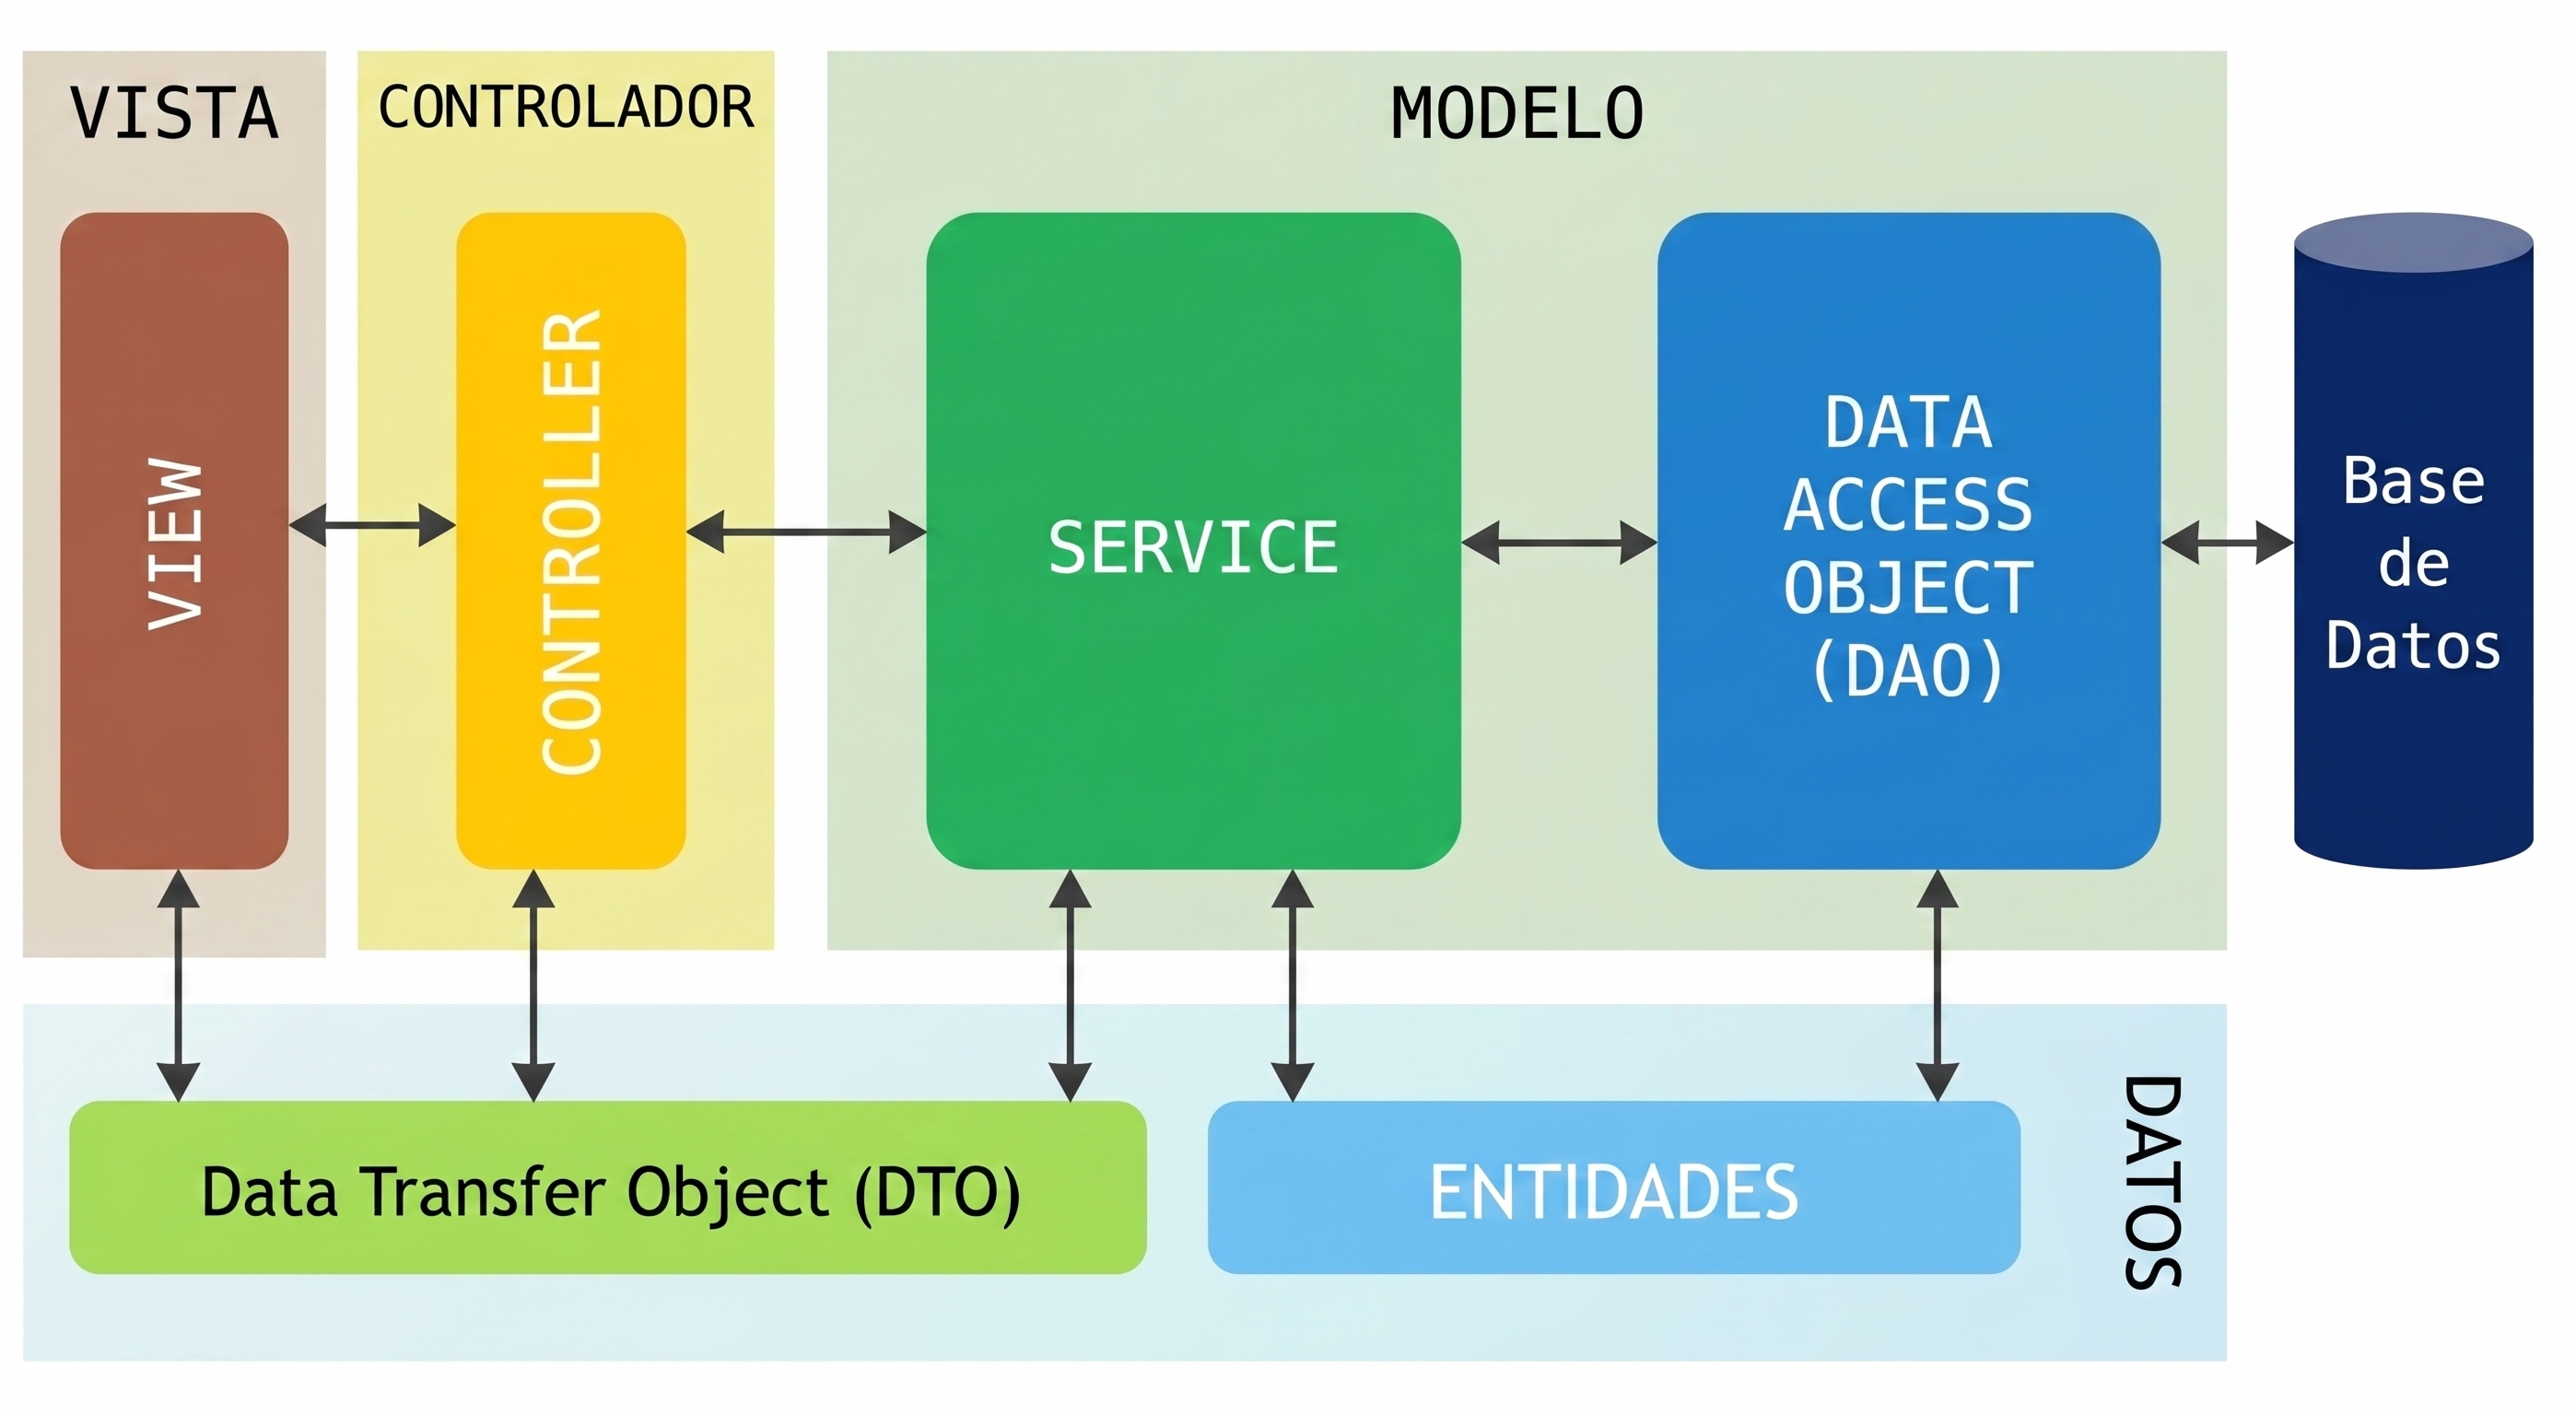
\includegraphics[width=0.80\linewidth]{assets/mermeid/PatronMVC.png}}{\textit{Fuente: Patrones de diseño DTO y Service, Eduardo Guzmán De los Riscos (guzman@lcc.uma.es)}}
\end{figure}
\par
\vspace{5mm}
La comunicación entre frontend y backend se realiza
exclusivamente mediante una API REST sobre HTTPS, autenticada con JWT. % chktex 13
El navegador del usuario nunca accede directamente a la base de datos: todas las
reglas de negocio, validaciones y comprobaciones de autorización residen en el
backend, lo que mantiene un perímetro de confianza claro y simplifica las
auditorías de seguridad.    
\begin{figure}[H]
    \centering
    \caption{Diagrama de arquitectura API RESTful}
    \copyrightbox[b]{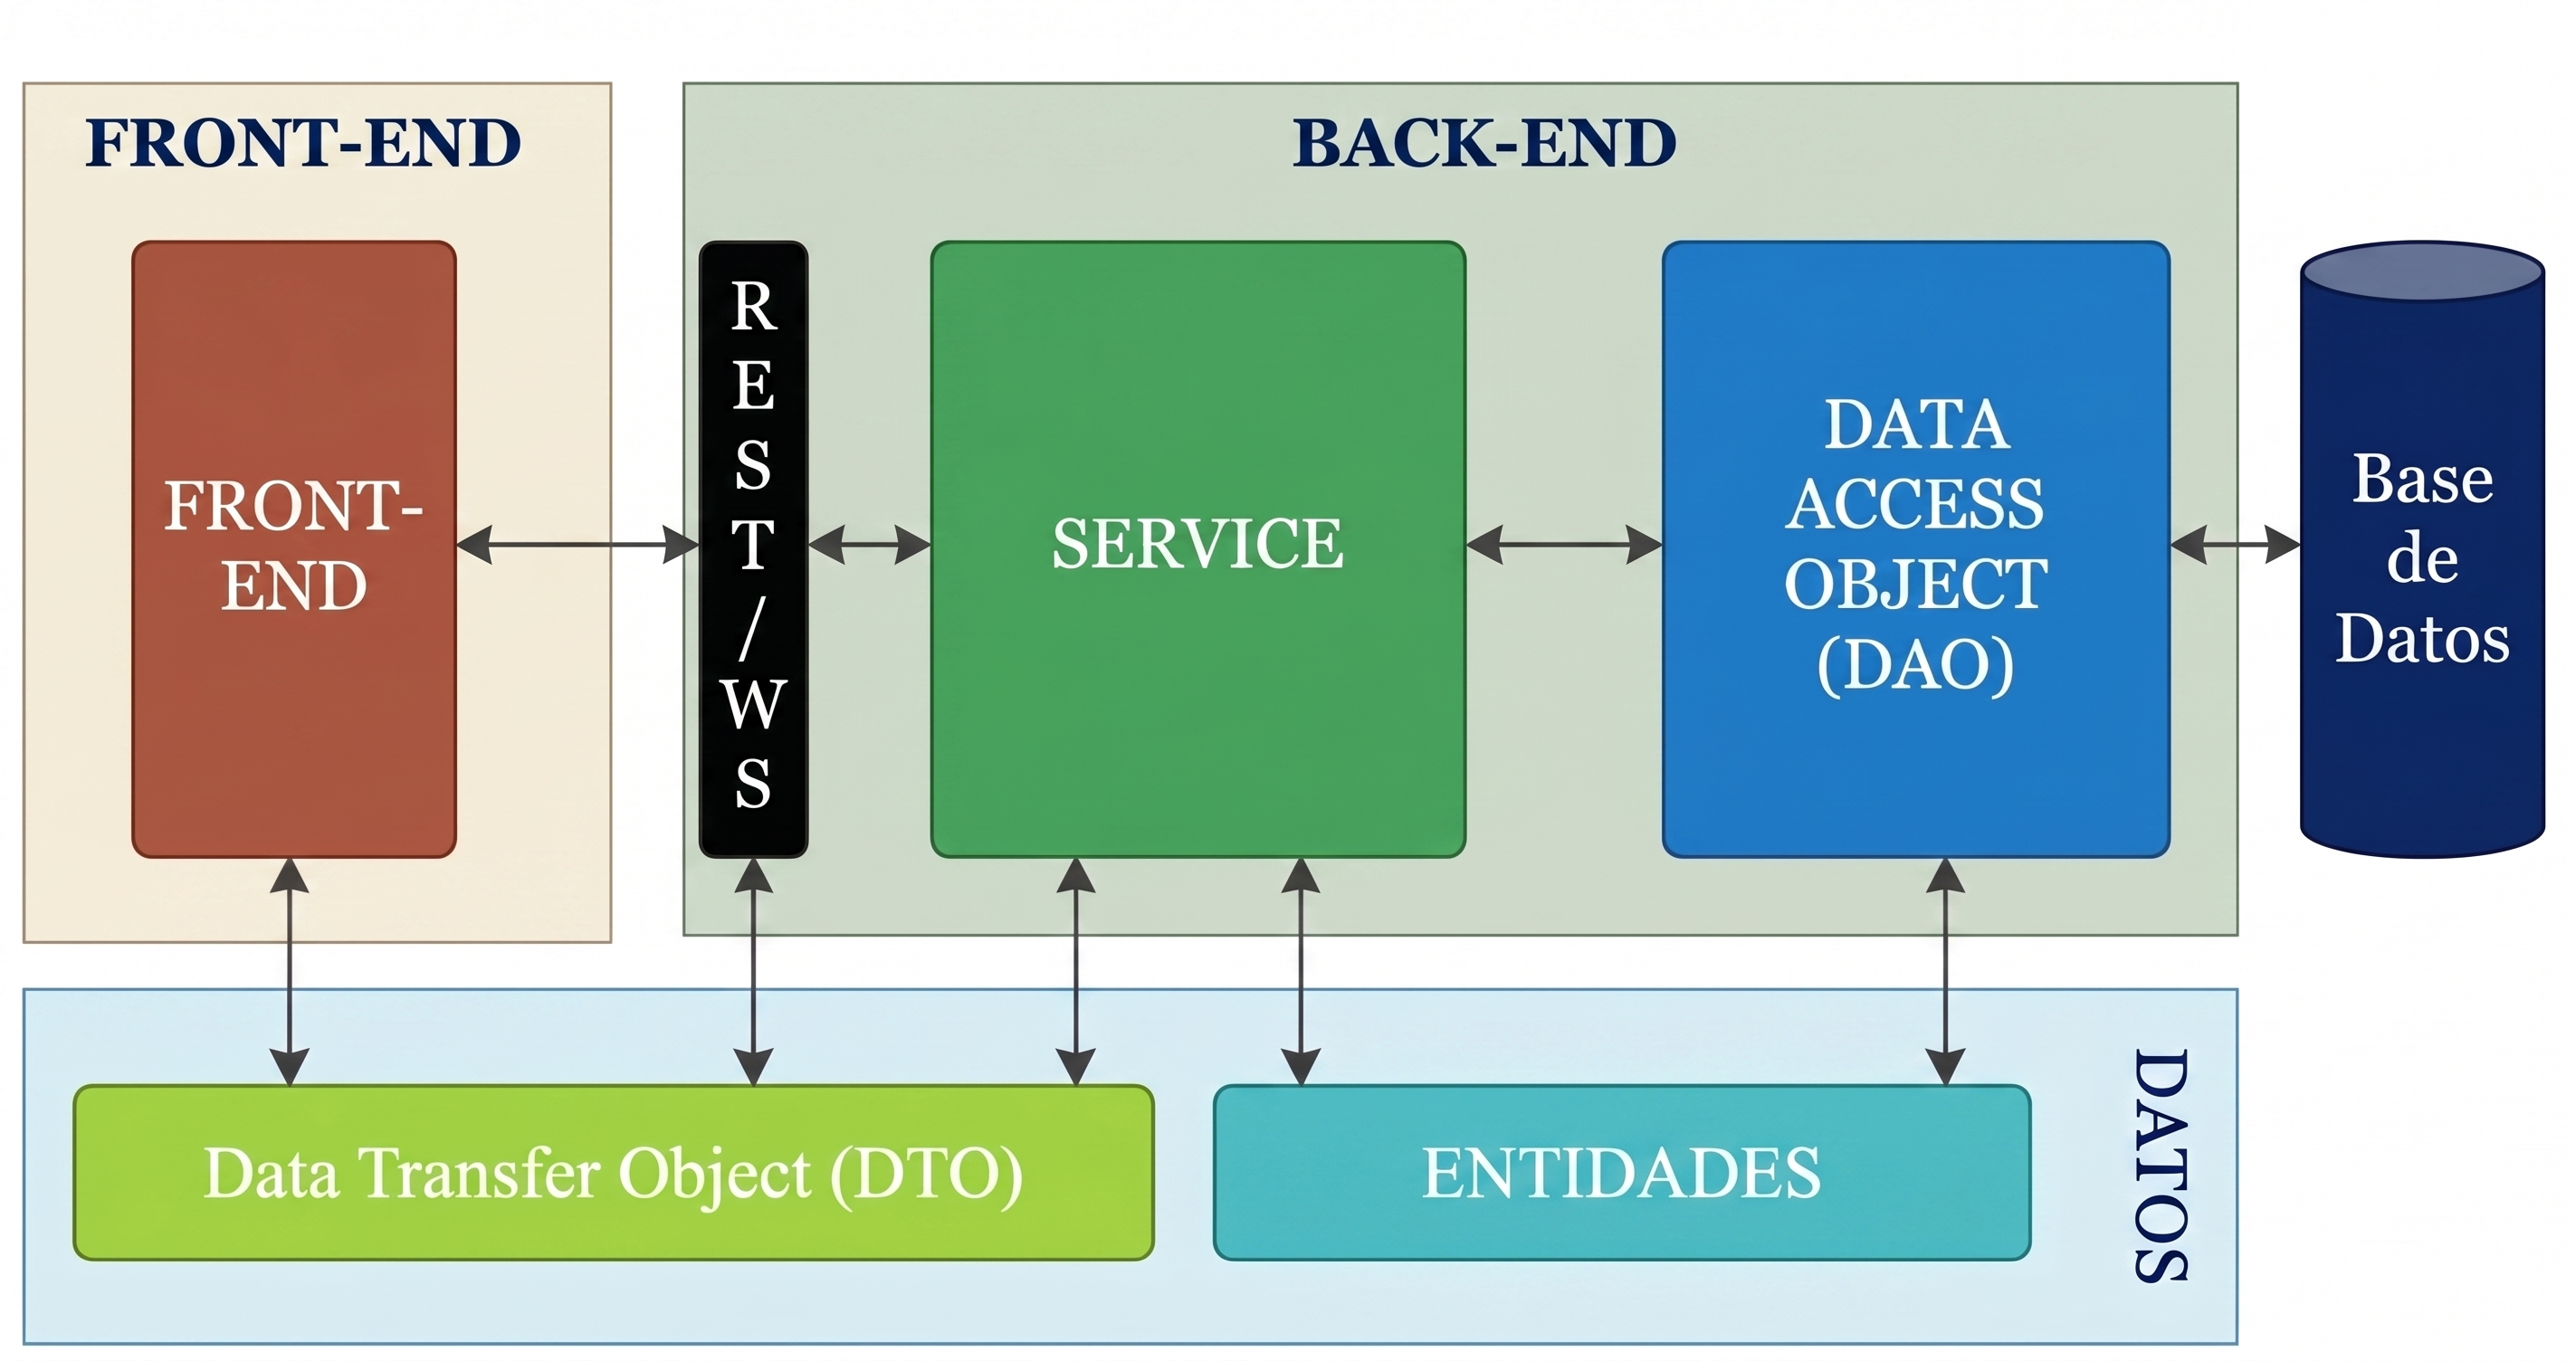
\includegraphics[width=0.80\linewidth]{assets/mermeid/ArquitecturaGeneral.png}}{\textit{Fuente: Patrones de diseño DTO y Service, Eduardo Guzmán De los Riscos (guzman@lcc.uma.es)}}
\end{figure}
\par
\vspace{5mm}
El conjunto se empaqueta mediante \textbf{Docker} y se despliega en \textbf{Render}, que
proporciona la infraestructura en la nube, el balanceo de carga, el
certificado TLS y la conexión privada entre el servicio web y la base de datos.
La gestoría fiscal externa, las entidades financiadoras y las autoridades
sanitarias son actores externos al sistema: interactúan con él de forma
indirecta, recibiendo informes exportados (CSV, PDF, JSON) generados desde la
aplicación.
\begin{figure}[H]
    \centering
    \caption{Diagrama de arquitectura general y fronteras del sistema}
    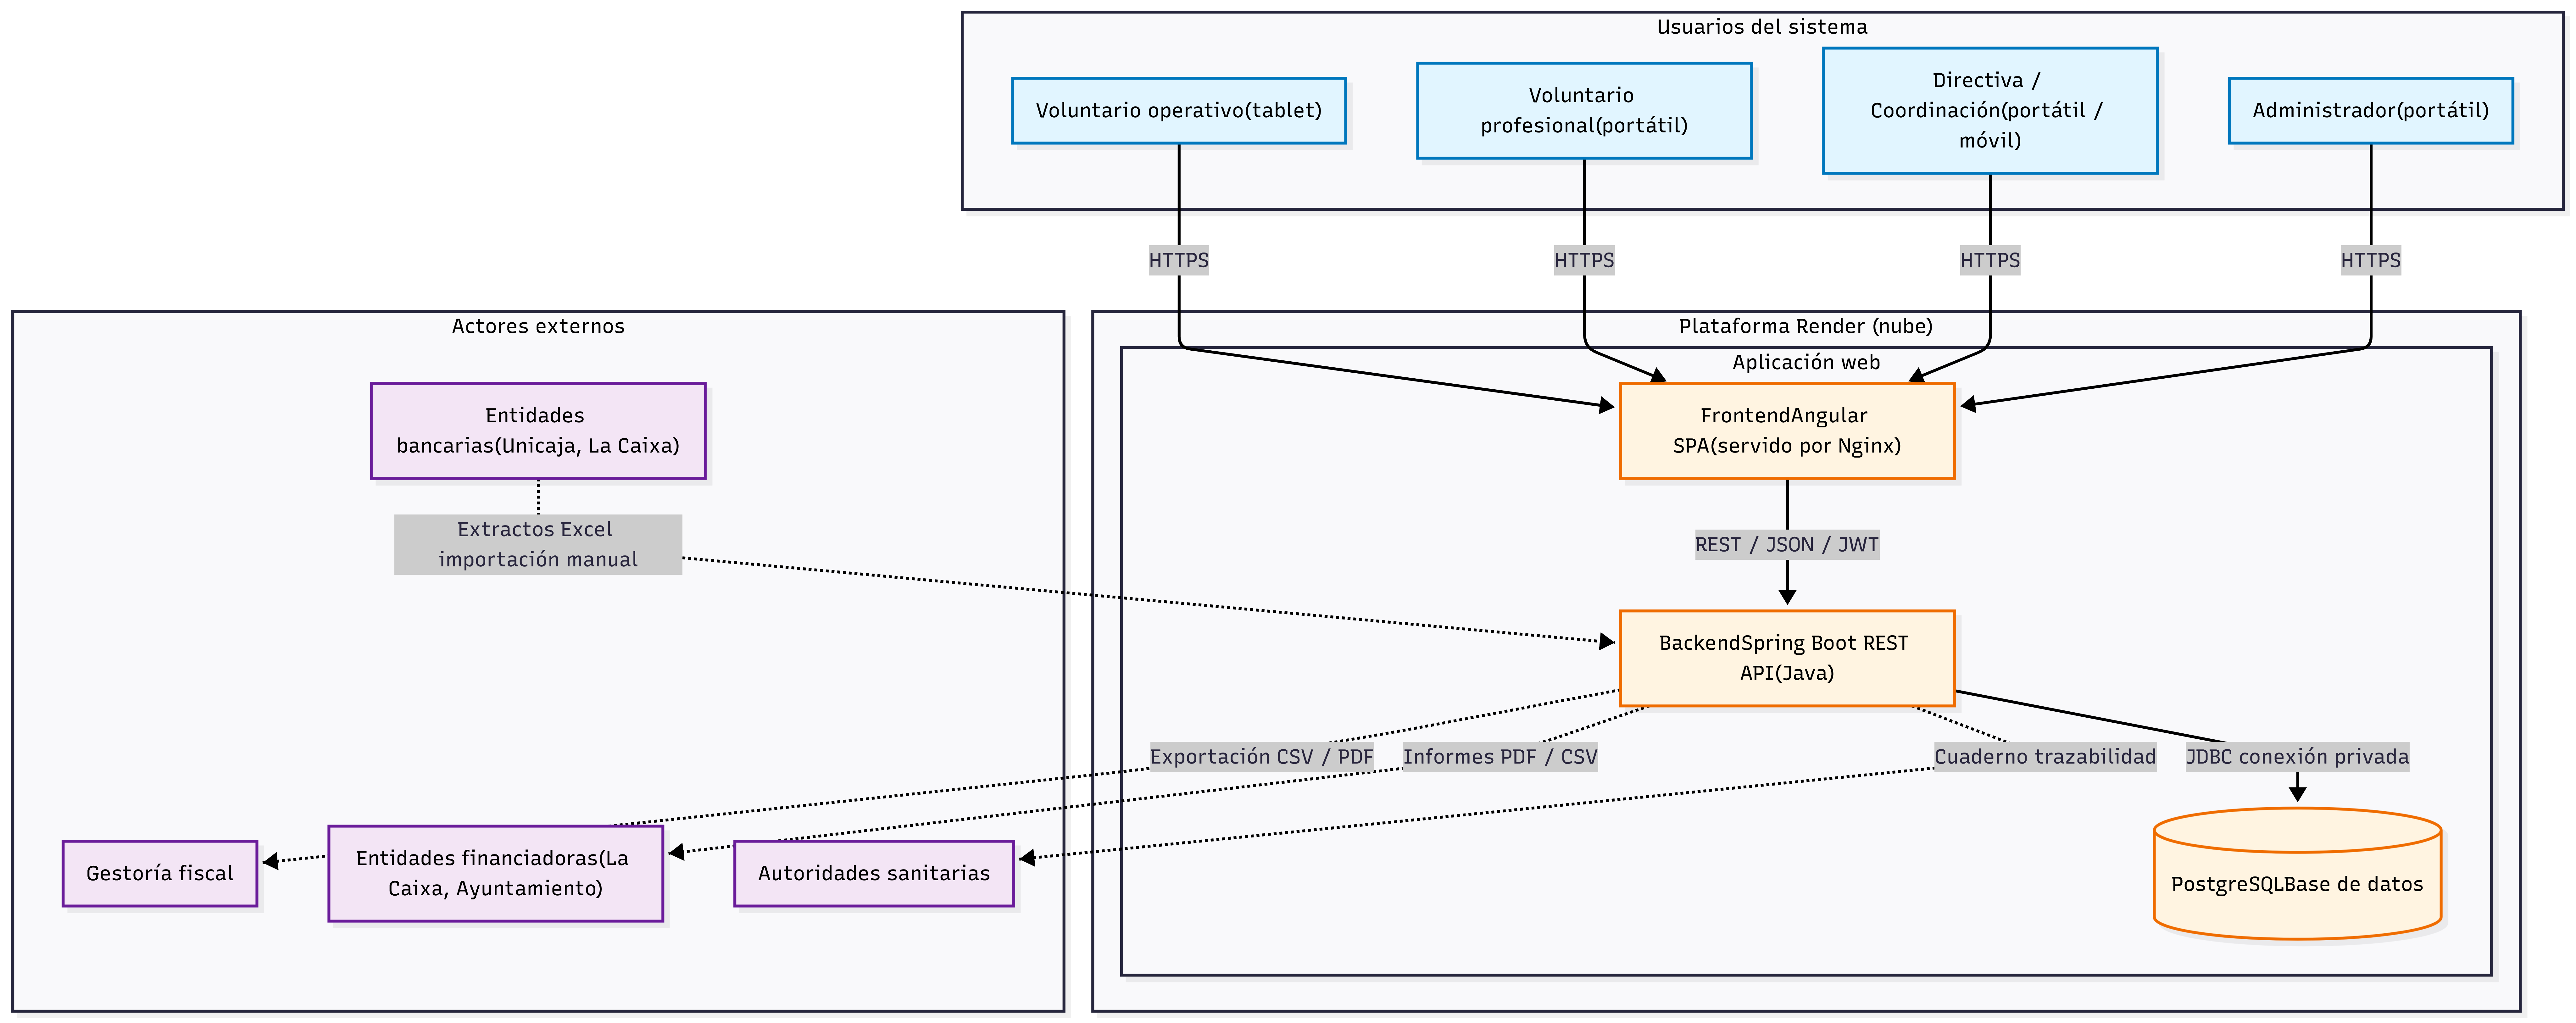
\includegraphics[width=1\linewidth]{assets/mermeid/Arquitectura-Fronteras-delSistema.png}
\end{figure}
\par
\vspace{5mm}
Las flechas de trazo continuo representan interacción en tiempo real mediada
por el sistema; las de trazo discontinuo representan flujos diferidos de
intercambio de información (importaciones manuales de extractos bancarios,
generación periódica de informes para terceros).


\subsection{Funciones del Producto}\hypertarget{section2.2}{anchor text}
A continuación se resume el alcance de cada una de las áreas funcionales en el sistema a un nivel 
suficiente para entender su propósito sin entrar en el detalle de cada operación.
\begin{itemize}
    \item \textbf{Gestión de cuentas y autenticación}. Permite crear, modificar y dar de baja
    cuentas de voluntario en el sistema, así como gestionar el inicio y cierre de
    sesión, la recuperación de contraseña y la protección frente a accesos no
    autorizados. Es la puerta de entrada al sistema: ninguna otra función está
    disponible sin haber atravesado este bloque.

    \item \textbf{Control de acceso y roles}. Implementa el sistema de permisos: define qué
    roles existen (administrador, operativo, profesional, puente, agente externo
    temporal), qué nivel de seguridad tiene cada voluntario para visualizar datos
    sensibles (\texttt{BÁSICO} o \texttt{PRIVILEGIADO}) y qué funciones específicas puede ejecutar
    cada uno (entregar ropa, agendar servicio, registrar gastos, leer notas
    psicológicas, importar extractos bancarios, etc.). Incluye el mecanismo de
    habilitación temporal que permite a la coordinación abrir puntualmente el
    acceso a un voluntario profesional sobre el expediente de un amigo concreto.

    \item \textbf{Gestión del amigo.} Mantiene el expediente de cada persona atendida con un
    modelo de \textbf{ficha progresiva} que escala según el nivel de confianza
    alcanzado: en el primer contacto sólo se registra el nombre; con la
    recurrencia se añaden alias, tallas y datos básicos; sólo tras una entrevista
    de profundidad se incorpora el DNI y los datos sensibles. Cada amigo dispone
    de un histórico completo.

    \item \textbf{Servicios y agendamiento.} Gestiona el catálogo de servicios que el centro
    ofrece: duchas, asistencia jurídica, médica, psicológica, podología,
    extranjería, educativa, entre otras y permite agendarlos con fecha, hora y voluntario
    asignado. Implementa control de capacidad por turno (por ejemplo, máximo
    cuatro duchas por turno para evitar cuellos de botella) y la regla de
    pre-requisito: sin agendamiento no se presta el servicio.

    \item \textbf{Inventario, entregas y lavandería.} El \textbf{armario general} opera como un stock
    impersonal: se registran las donaciones recibidas, se controla el inventario
    por tipo y talla, y cada entrega a un amigo decrementa automáticamente el
    stock aplicando reglas de frecuencia configurables (por ejemplo, un par de
    zapatillas cada tres meses para el mismo amigo). No se opera de forma personal: el centro no recibe ropa 
    propia del amigo, la lava y se la devuelve a la misma persona; se va rotando la ropa a necesidad del amigo que la solicite.

    \item \textbf{Trazabilidad alimentaria.} Implementa el cuaderno de entradas y salidas
    exigido por la Ley 1/2025. Registra el origen de cada alimento (compra
    propia, donación de entidad con convenio, donación particular, etc.), su lote y
    fecha de caducidad, su clasificación según prioridad legal de
    aprovechamiento, las verificaciones de higiene del producto y del lugar de
    almacenamiento, y la temperatura de salida en el caso de productos
    refrigerados. Asocia tickets, albaranes y convenios (cuando existen), y permite
    generar el cuaderno completo en formato apto para inspección sanitaria.

    \item \textbf{Gestión contable.} Reproduce y automatiza el flujo que la contabilidad 
    que se lleva hoy manualmente en Excel. Mantiene un plan de cuentas
    parametrizable (por ejemplo, códigos como 600 para gastos de comunidad, 5720 para bancos,
    6260 para servicios bancarios\ldots), permite importar los extractos bancarios en formato Excel, 
    y aplica reglas de mapeo automático que
    asocian conceptos recurrentes a las cuentas correspondientes, generando los asientos de diario sin intervención
    manual. 
    \par
    Diferencia los flujos de \textbf{tarjeta bancaria} y \textbf{caja chica} en
    efectivo, categoriza cada gasto como propio de la Casa, del amigo o mixto, y
    permite vincularlo opcionalmente a un amigo o a un servicio concreto para
    obtener trazabilidad por persona (esto ayuda a responder preguntas del tipo \textit{``¿cuánto hemos gastado en Francisco este
    semestre?''}). % chktex 38

    \item \textbf{Reportes, informes y visualización.} Centraliza la salida de datos del
    sistema. Ofrece un panel visual con los indicadores que la directiva consulta
    con mayor frecuencia (gastos por categoría, número de servicios prestados al
    mes, costes de alimentación, número de cafés servidos), genera informes
    numéricos exactos por mes, semestre o año para
    presentar a entidades financiadoras, y permite exportar la información en
    PDF, CSV y JSON. Soporta filtros y consultas \textit{ad-hoc}\footnote{Una \textit{consulta ad-hoc} (del latín ``para esto'') es una búsqueda o informe de datos creado desde cero para responder a una pregunta puntual e inmediata.} por amigo, servicio, % chktex 13
    periodo, voluntario o cuenta contable.

    \item \textbf{Puente analógico-digital y carga inicial.} Reconoce que una parte
    significativa del voluntariado opera con papel y debe seguir pudiendo
    hacerlo. El sistema prepara planillas con exactamente los mismos campos que
    las entidades de la base de datos, de modo que un voluntario
    analógico rellena a mano y otro voluntario carga después esos datos al
    sistema. Adicionalmente, soporta la importación masiva de los datos
    históricos contenidos hoy en las hojas Excel de la coordinación y la
    contabilidad, validando duplicados y errores de formato durante la carga.
\end{itemize}
\par
\vspace{5mm}

\begin{figure}[H]
    \centering
    \caption{Organización funcional del sistema}
    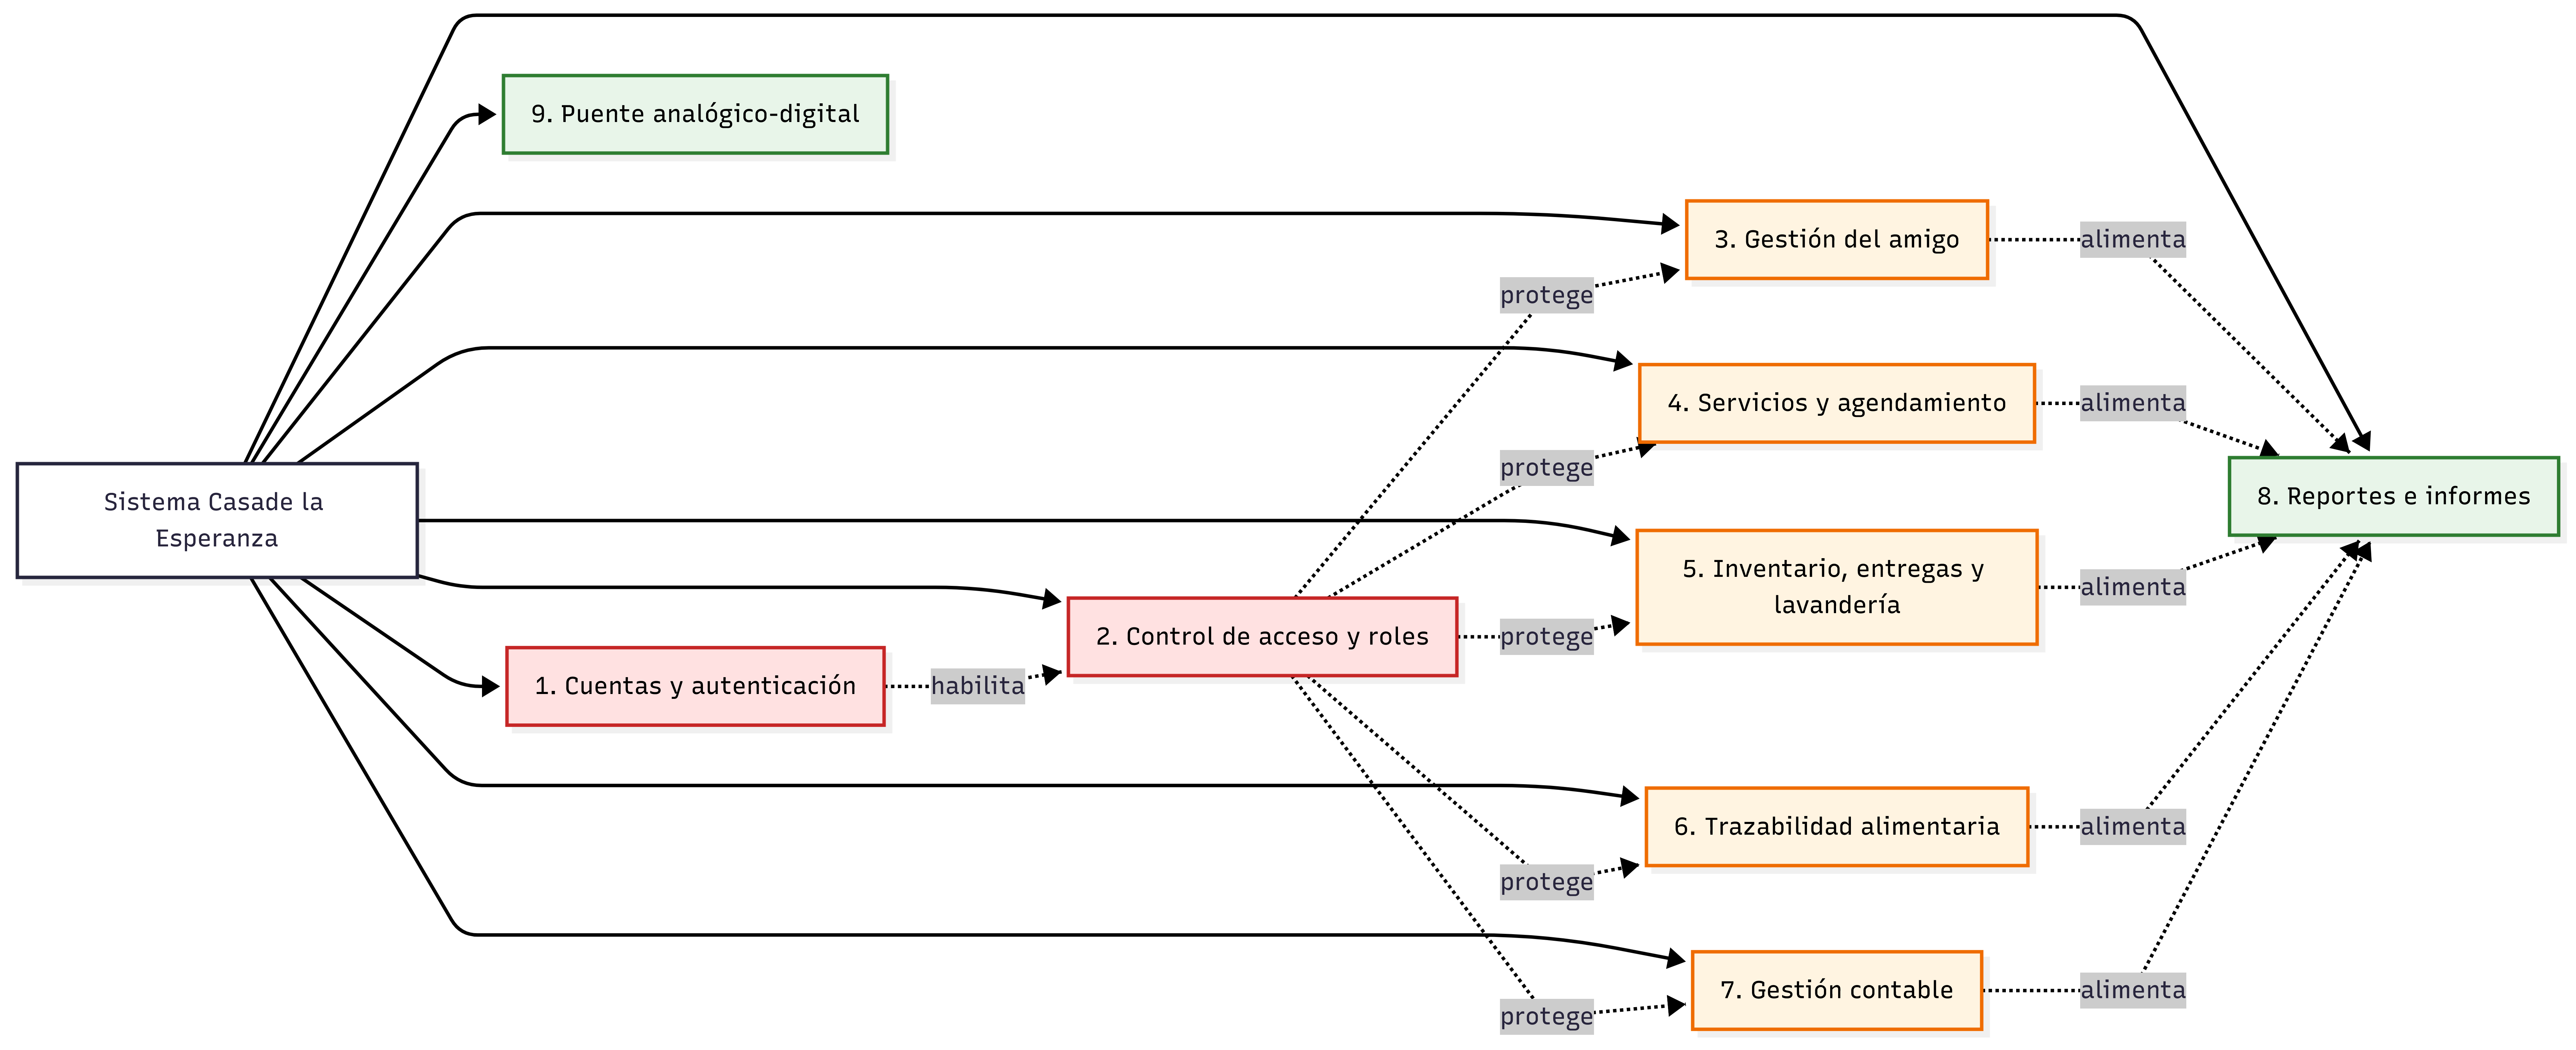
\includegraphics[width=1\linewidth]{assets/mermeid/organizacionFuncional.png}
\end{figure}
\par
\vspace{5mm}

\subsection{Requisitos Futuros}\label{section_RequisitosFuturos}
Esta sección propone mejoras y extensiones del sistema que no forman parte del
alcance de la versión inicial pero que se han identificado durante el proceso
de captura de requisitos como deseables a medio o largo plazo.

\begin{itemize}
    \item \textbf{Sistema de notificaciones automáticas.} Envío proactivo de avisos a
    voluntarios y miembros de la directiva ante eventos relevantes: alimentos
    próximos a caducar, stock de armario por debajo de umbral, citas profesionales
    del día siguiente, gastos pendientes de aprobación, fin de vigencia de un
    convenio de donación. Los canales contemplados son correo electrónico y
    WhatsApp.

    \item \textbf{Trazabilidad de comunicaciones externas extendida.} Aunque el registro
    manual de comunicaciones vinculadas al amigo (correos a policía,
    ayuntamiento, citas externas) está contemplado como funcionalidad de la
    versión inicial (ver \hyperlink{RF3.6}{RF3.6}), la integración automática con la % chktex 2
    bandeja de correo de modo que los correos enviados o
    recibidos relacionados con un amigo se asocien automáticamente a su perfil,
    con análisis de remitente, destinatario y palabras clave se considera una
    mejora futura.

    \item \textbf{Diseño responsive multi-dispositivo.} La versión actual del proyecto esta destinada a ser una aplicación web 
    principalmente accesible y operable desde un ordenador. Diseño responsive para acomodar dispositivos de distintas dimensiones 
    como tablets o móviles es una solicitud real, pero fuera del alcance inicial.

    \item \textbf{Migración de la base de datos.} Si el
    volumen de datos crece significativamente (por ejemplo, si la asociación
    amplía su radio de acción o si se incorporan otras delegaciones), puede
    ser necesario migrar de la instancia PostgreSQL gestionada por Render a
    una solución de mayor capacidad, replicación geográfica o particionado.

    \item \textbf{Internacionalización.} La versión inicial está disponible únicamente en
    español (España). La incorporación de inglés (US/UK) facilitaría la
    interacción con voluntarios y amigos no hispanohablantes en la propia
    interfaz, especialmente en los formularios que se cumplimentan junto al
    amigo.

    \item \textbf{RF6.x Gestión de convenios con entidades donantes} \\
    El sistema debe permitir registrar y mantener los convenios de donación
    firmados con entidades aportantes regulares (Mercadona, Bancosol, etc.).
    \begin{description}
        \item[-] El sistema avisa visualmente cuando un convenio se aproxima a su
        fecha de vencimiento (por defecto, 30 días antes).
    \end{description}
    \par
    Este requisito formaba parte del DGR DOC001 pero cuando se revisó con el cliente, a pesar que la Ley 1/2025 exige 
    en el articulo 6.4.b) que los agentes de la cadena alimentaria (como Mercadona) promuevan convenios para donar sus excedentes de alimentos a  % chktex 10 
    asociaciones como la Casa de la Esperanza, se decidió dejar fuera ya que no está en su interés tener esta clase de convenios por el momento.
\end{itemize} % chktex 17
\section{Atributos del Sistema}
Este capítulo presenta los atributos de calidad que el sistema debe satisfacer, 
las llamadas \textit{-ilities}, las restricciones que limitan las decisiones de
diseño y desarrollo, y las alternativas tecnológicas que se evaluaron antes de
optar por el desarrollo a medida. Los atributos enumerados aquí se concretarán
posteriormente en requisitos no funcionales medibles en el capítulo 7.

\subsection{Atributos de Calidad}
\begin{itemize}
    \item \textbf{Confidencialidad $-$ Prioridad: Crítica.} 
    Atributo derivado de la seguridad pero específicamente referido a la
    protección frente a divulgación no autorizada de datos. Las ``notas privadas''
    de los acompañamientos profesionales sólo deben ser visibles para voluntarios con el rol y 
    nivel correspondiente.

    \item \textbf{Fiabilidad} 
    Capacidad del sistema para funcionar correctamente bajo 
    condiciones normales de uso, minimizando fallos y tiempos de inactividad. Se materializa en la
    integridad referencial de la base de datos, la atomicidad transaccional de
    las operaciones que afectan a múltiples entidades (por ejemplo, una entrega
    de ropa que decrementa el stock y crea un registro histórico) y la copia de
    seguridad periódica con prueba de restauración.

    \item \textbf{Trazabilidad} 
    La trazabilidad es una de las 
    motivaciones centrales del proyecto. Se materializa en el registro inmutable de creaciones,
    modificaciones y eliminaciones (con identificador del voluntario y marca de
    tiempo), en el histórico de cambios de las entidades sensibles.

    \item \textbf{Cumplimiento legal} 
    El sistema debe satisfacer las exigencias documentales y de trazabilidad que
    imponen dos marcos legales: Ley 1/2025.

    \item \textbf{Mantenibilidad.}  
    Se materializa en una arquitectura por capas con responsabilidades bien delimitadas, código
    estructurado en módulos cohesionados, documentación técnica actualizada,
    cobertura de pruebas suficiente para detectar regresiones.

    \item \textbf{Escalabilidad}
    El volumen de datos previsto es modesto: la coordinación estima un universo
    de menos de cien amigos atendidos simultáneamente, en torno a una veintena
    de voluntarios activos, y un volumen de transacciones diarias del orden de
    decenas (no de miles ni de millones). El sistema debe funcionar
    correctamente en este orden de magnitud sin necesidad de optimizaciones
    costosas, pero la arquitectura debe permitir un crecimiento moderado sin reescritura.

    \item \textbf{Disponibilidad}
    Una caída de varias horas durante la madrugada no impide la operativa. Sin embargo, debe
    estar disponible durante los turnos de actividad del centro. Con el plan adecuado de despliegue
    podemos asegurar una disponibilidad del 99.5\% durante las horas de actividad.
\end{itemize}


\subsection{Restricciones}
Las restricciones limitan las decisiones de diseño y desarrollo del sistema.

\subsubsection{Restricciones Tecnológicas}
\begin{itemize}
    \item \textbf{Backend en Java con Spring Boot:} La elección responde al conocimiento
    previo del desarrollador, a la madurez del ecosistema Spring para
    aplicaciones empresariales y a la disponibilidad de Spring Security como
    base sólida para la implementación de autenticación y autorización.

    \item \textbf{Frontend en Angular:} La elección responde a tres factores:
    \par
    \vspace{5mm}
    Primero,
    la idoneidad del framework
    para aplicaciones de formulario intensivas como la presente.
    \par
    \vspace{5mm}
    Segundo, a la sinergia probada con backend Spring
    Boot: Angular y Spring Boot constituyen una combinación full-stack
    ampliamente adoptada en entornos de producción, en la que el contrato
    entre ambos lados es una API REST sobre HTTPS y la seguridad se articula
    mediante Spring Security con tokens JWT validados en cada petición. Esta
    arquitectura permite que el frontend opere como una aplicación
    desacoplada (\textit{Single Page Application}) que consume servicios sin estado,
    lo que facilita el despliegue independiente de cada capa, la
    escalabilidad horizontal y la sustitución del frontend en el futuro sin
    reescritura del backend. 
    \par
    \vspace{5mm}
    Tercero, al ecosistema maduro de
    herramientas que Angular proporciona: enrutamiento, formularios
    reactivos con validación, interceptores HTTP (ideales para inyectar el
    token JWT en cada petición y para gestionar errores de autorización de
    forma centralizada), y soporte de pruebas unitarias y end-to-end
    integrado. La sinergia técnica entre Angular y Spring Boot está
    ampliamente documentada en la literatura de arquitectura full-stack
    contemporánea [10].
    % TODO:
    % Deberíamos detallar la sinergia con sequence diagrams en algún Apéndice de acuerdo a los flujos en:
    % https://medium.com/@sanikapatil0213/how-angular-and-spring-boot-form-a-production-ready-full-stack-architecture-1bd63f3a84a2

    \item \textbf{Base de datos PostgreSQL:} La elección responde a su integración nativa con Render además de 
    la disponibilidad de cifrado de columna nativo (pgcrypto) para proteger los datos sensibles, y su
    cumplimiento estricto del estándar SQL\@.

    \item \textbf{Empaquetado mediante Docker.} Garantiza reproducibilidad del entorno entre desarrollo, 
    pruebas y producción además de permitir una BD PostgreSQL local desechable idéntica al de producción sin instalar nada en el sistema.

    \item \textbf{Despliegue en Render.} Plataforma de alojamiento gestionado en la
    nube. Implica aceptar las restricciones de los planes contratados. Sin embargo, ofrece 
    un nivel de suscripción gratuito para pruebas o demos (30 días máximos). 

    \item \textbf{Comunicación frontend-backend exclusivamente mediante API REST sobre HTTPS.}
\end{itemize}


\subsubsection{Restricciones de Hardware y Entorno}
\begin{itemize}
    \item El sistema debe ser accesible desde dispositivos con navegadores web modernos, incluyendo 
    ordenadores de escritorio, portátiles, tabletas y smartphones. No se requiere compatibilidad con 
    navegadores obsoletos.
    \item El sistema debe operar en condiciones de conectividad doméstica
    estándar, es decir, no presupone del uso de un ancho de banda empresarial para su funcionamiento correcto.
\end{itemize}


\subsubsection{Restricciones Operativas}
\begin{itemize}
    \item \textbf{Auditoría obligatoria de operaciones sensibles.} Toda creación,
    modificación o eliminación de información relevante (especialmente datos
    sensibles, entregas, gastos, asientos contables y entradas alimentarias)
    debe quedar registrada con identificador del voluntario, marca de
    tiempo y, en caso de modificación, valor anterior.

    \item \textbf{Idioma único: español.} La interfaz, los mensajes de error, la
    documentación de usuario y los informes generados se producen en español de España.
\end{itemize}



\subsection{Alternativas Consideradas}
Antes de optar por el desarrollo a medida, durante las entrevistas se
evaluaron explícita o implícitamente varias alternativas. A continuación se
documentan las consideradas y los motivos que llevaron a descartarlas.


\subsubsection{Continuar con Hojas de Cálculo en Google Drive}
La alternativa más sencilla y económica habría sido sistematizar las hojas
de cálculo actuales en una estructura compartida en Google Drive. Esta
opción se descartó por \textbf{concurrencia limitada} (aunque \textit{Google Sheets} permite edición
simultánea, no soporta de forma fiable la operación concurrente de
múltiples voluntarios sobre las mismas filas), \textbf{carga manual elevada}, \textbf{dificultad para generar informes complejos} 
debido a la descentralización de la información en múltiples hojas, y \textbf{riesgo de pérdida de datos} por errores humanos e 
\textbf{imposibilidad de cumplir la Ley 1/2025} de forma cómoda y fiable.


\subsubsection{CiviCRM}
CiviCRM es un CRM de código abierto orientado a organizaciones sin ánimo
de lucro gratuito. Fue propuesto por uno de los
colaboradores de la directiva y evaluado durante la segunda entrevista más impone 
uso sistema operativo Linux que no se posee ni se desea. Además, gira en torno a
donantes, contribuciones y campañas de captación de fondos; su modelo
no se ajusta de forma natural al concepto de ``amigo con ficha
progresiva por nivel de confianza'' que es central al proyecto.


\subsubsection{Salesforce}
Salesforce ofrece una variante de su plataforma orientada a entidades sin
ánimo de lucro, con descuentos significativos y dotación gratuita inicial
de licencias (NPSP / Power of Us). Se evaluó y se descartó por los
siguientes motivos:
\begin{itemize}
    \item Aunque la dotación inicial es
    gratuita, es altamente limitada en cuanto al número de usuarios. 
    \item La ampliación de licencias, el almacenamiento adicional y el
    soporte de funcionalidades avanzadas implican costes recurrentes elevados.
    \item Ofrece una
    funcionalidad muy superior a la requerida, gran parte de la cual no
    se aprovecharía, lo que se traduce en una interfaz innecesariamente
    compleja para los voluntarios.
    \item Imposibilidad de unificar dominios de trazabilidad alimentaria
   y la contabilidad operativa para
    cuentas y mapeo de extractos bancarios; escapan al alcance natural de
    un CRM y exigirían integraciones con sistemas adicionales.
\end{itemize}


\subsubsection{ERPs de Código Abierto}
Se descartaron por motivos similares a los de CiviCRM y Salesforce: sobre-dimensionamiento,
inadecuación conceptual al dominio y dificultad para implementar el
módulo específico de trazabilidad alimentaria. Los consultados fueron ERPNext y Dolibarr.


\subsubsection{Conclusión}
La combinación de tres factores hace inviables las alternativas evaluadas y
justifica el desarrollo a medida:
\begin{enumerate}
    \item La necesidad de implementar el \textbf{módulo de trazabilidad alimentaria de la
    Ley 1/2025} específico del dominio de ayuda comunitaria en cualquier
    solución elegida.

    \item La necesidad de unificar en una misma aplicación la gestión de personas,
    servicios, inventario, alimentación y contabilidad, lo que ningún
    producto comercial ofrece de forma nativa.

    \item La restricción presupuestaria que excluye soluciones SaaS de coste
    mensual significativo.
\end{enumerate}
\section{Descripción de Participantes y Usuarios}
Para diseñar un sistema efectivo es necesario identificar a todas las partes
afectadas por el proyecto y comprender sus necesidades reales. Este capítulo
distingue entre \textbf{participantes} (personas u organizaciones afectadas por el
proyecto pero que no son usuarios directos del sistema) y \textbf{usuarios} (personas
que interactúan directamente con la aplicación), describe sus perfiles, presenta
una visión general del producto desde la perspectiva de cada uno, detalla el
entorno de despliegue, recoge las suposiciones y dependencias del proyecto y
aborda los aspectos económicos.

\subsection{Resumen de los Participantes}
A continuación se enumeran las partes que se ven afectadas por el proyecto sin
ser necesariamente usuarios directos de la aplicación.

\vspace{5mm}

\begin{longtable}[]{@{}
    % Metadatos de la tabla
        p{0.28\columnwidth}
        p{0.22\columnwidth}
        p{0.50\columnwidth}@{}}

    \caption{Resumen de Participantes} \\

    % Configuración de la tabla para repetir encabezados en cada página
    \toprule
    \textbf{Participante} & \textbf{Naturaleza} & \textbf{Implicación en el proyecto} \\
    \midrule
    \endfirsthead % chktex 1

    \toprule
    \textbf{Participante} & \textbf{Naturaleza} & \textbf{Implicación en el proyecto} \\
    \midrule
    \endhead % chktex 1

    \midrule
    \multicolumn{2}{r}{\small\emph{Continúa en la siguiente página}} \\
    \endfoot % chktex 1

    \bottomrule
    \endlastfoot % chktex 1

    % Cuerpo de la tabla
    \textbf{Coordinación de la Casa de la Esperanza} & Cliente / Usuario &
    Promotor del proyecto, principal fuente de requisitos y usuario
    administrador del sistema (Ezequiel). \\
    \midrule

    \textbf{Directiva de la asociación} & Cliente / Usuario & Toma
    decisiones estratégicas sobre la asociación; consume informes y datos
    agregados del sistema. Incluye contabilidad (Miguel) y otros
    responsables de área. \\
    \midrule

    \textbf{Voluntariado operativo} & Usuario & Conjunto de voluntarios que
    cubren turnos en el centro: café, ropa, duchas, lavandería, recepción.
    Heterogéneo en cuanto a alfabetización digital. \\
    \midrule

    \textbf{Voluntariado profesional} & Usuario & Profesionales (abogados,
    médicos, psicólogos, podólogos, asistentes en extranjería) que prestan
    servicio especializado de forma puntual o regular. \\
    \midrule

    \textbf{Amigos atendidos} & Beneficiario / Sujeto de datos & Personas en
    situación de vulnerabilidad atendidas por la asociación. No son usuarios
    del sistema, pero sus datos personales constituyen el núcleo de la
    información gestionada. \\
    \midrule

    \textbf{Gestoría fiscal externa} & Tercero receptor & Recibe la
    información contable que la asociación le remite para la presentación de
    obligaciones fiscales. Interactúa con el sistema de forma indirecta a
    través de exportaciones. \\
    \midrule

    \textbf{Entidades financiadoras} & Tercero receptor & Reciben informes
    de actividad y de gasto con destino a la justificación de subvenciones.
    Incluyen La Caixa, Ayuntamiento de Málaga y otras entidades públicas y
    privadas. \\
    \midrule

    \textbf{Autoridades sanitarias} & Tercero receptor & Receptoras
    eventuales del cuaderno de trazabilidad alimentaria en caso de
    inspección, conforme a la Ley 1/2025. \\
    \midrule
    
    \textbf{Entidades donantes con convenio} & Tercero & Bancosol, Mercadona
    y otras entidades que donan alimentos o bienes a la asociación bajo
    acuerdos formales. \\
    \midrule

    \textbf{Donantes particulares} & Tercero & Personas que
    realizan donaciones puntuales (alimentos, ropa, dinero) sin convenio
    formal. \\
    \midrule

    \textbf{Equipo de desarrollo} & Proveedor & Responsable del desarrollo,
    despliegue y mantenimiento del sistema. Compuesto por un único
    desarrollador en la fase actual del proyecto. \\
    \midrule
    
    \textbf{Render (proveedor de infraestructura)} & Proveedor técnico &
    Plataforma de alojamiento gestionado en la nube donde se despliega la
    aplicación. \\
\end{longtable}

\newpage

\subsection{Perfiles de los Participantes}
A continuación se detallan los perfiles de los participantes que no son
usuarios directos del sistema pero cuyas necesidades, restricciones o
expectativas afectan al diseño.

\subsubsection{Coordinación}
\begin{itemize}
    \item \textbf{Representante:} Ezequiel.
    
    \item \textbf{Responsabilidades:} Dirección operativa diaria de la Casa de la Esperanza,
    relación con voluntariado, decisión última sobre admisión y trato a los
    amigos, autorización de compras significativas, relación con donantes y
    entidades externas.
    
    \item \textbf{Necesidades respecto al sistema:} Visibilidad completa sobre toda la
    operación, trazabilidad por persona y
    por universo, capacidad de delegar acceso granular a otros voluntarios
    manteniendo el control sobre datos sensibles, herramientas que reduzcan la
    carga manual y permitan rendir cuentas a la directiva y a financiadores con
    datos exactos en lugar de porcentajes aproximados
\end{itemize}


\subsubsection{Directiva (Contabilidad)}
\begin{itemize}
    \item \textbf{Representante:} Miguel 
    
    \item \textbf{Responsabilidades:} Contabilidad de la asociación, relación con la
    gestoría fiscal, validación de gastos, control financiero, informes a
    órganos de gobierno y financiadores.
    
    \item \textbf{Necesidades respecto al sistema:} Importación automatizada de extractos
    bancarios, mapeo de conceptos a cuentas contables, generación de asientos
    sin trabajo manual repetitivo, acceso desde el domicilio a los datos
    contables, capacidad de consulta autónoma sin depender de la gestoría,
    trazabilidad de gasto por persona atendida.
\end{itemize}


\subsubsection{Gestoría Fiscal Externa}
\begin{itemize}
    \item \textbf{Responsabilidades:} Cierre fiscal de la asociación.
    
    \item \textbf{Necesidades respecto al sistema:}  Recibir información estructurada,
    exportable y trazable de la actividad económica de la asociación.
    
    \item \textbf{Restricciones:} El sistema debe poder exportar a
    formatos estándar (CSV, PDF) compatibles con el flujo de la gestoría. La
    gestoría no es un usuario del sistema y no se contempla integración
    técnica en esta versión.
\end{itemize}


\subsubsection{Autoridades Sanitarias}
\begin{itemize}
    \item \textbf{Necesidades respecto al sistema:} En caso de inspección, recibir el
    cuaderno de entradas y salidas alimentarias con la trazabilidad completa
    exigida por la Ley 1/2025 (lotes, caducidades, temperaturas, prioridad
    legal, convenios).
    
    \item \textbf{Implicaciones de diseño:} El cuaderno debe ser exportable en formato
    imprimible y debe garantizar la inmutabilidad de los registros una vez
    cerrado el periodo correspondiente.
\end{itemize}


\subsubsection{Equipo de Desarrollo}
\begin{itemize}
    \item \textbf{Composición actual:} Un único desarrollador.
    
    \item \textbf{Implicaciones de diseño:} La arquitectura debe favorecer la
    mantenibilidad por una sola persona, la simplicidad operativa, el uso de
    herramientas y librerías ampliamente documentadas y la cobertura de
    pruebas suficiente para detectar regresiones sin necesidad de equipos de
    QA dedicados.
\end{itemize}


\newpage

\subsection{Perfiles de los Usuarios}
Los usuarios directos del sistema se agrupan en cinco perfiles, cada uno con
un rol asociado en el modelo de control de acceso definido en RF2.1. La
relación entre perfil de usuario y rol no es uno a uno: un mismo voluntario
puede acumular varios roles si su nivel de implicación lo justifica.

\subsubsection{Adminitrador}
\begin{itemize}
    \item \textbf{Rol del sistema:} \texttt{ADMIN}.
    
    \item \textbf{Quién asume este perfil:} Coordinación (Ezequiel) y,
    personas de máxima confianza de la directiva (por ejemplo, Miguel).
    
    \item \textbf{Permisos:}
    \begin{itemize}
        \item Crear, editar y desactivar cuentas de voluntario.
        \item Asignar y revocar roles, niveles de seguridad y funciones específicas.
        \item Habilitar accesos temporales a voluntarios profesionales sobre amigos concretos.
        \item Acceso completo a todos los datos del sistema.
        \item Acceso a la gestión financiera y creación de asientos contables.
        \item Exportación de informes para entidades financiadoras y autoridades.
        \item Acceso al registro de auditoría.
    \end{itemize}
\end{itemize}


\subsubsection{Voluntario Operativo}
\begin{itemize}
    \item \textbf{Rol del sistema:} \texttt{OPERATIVO}.
    
    \item \textbf{Quién asume este perfil:} El voluntariado del centro;
    personas que cubren turnos de mañana o tarde en tareas como recepción,
    café, ropa, duchas, lavandería y registro de servicios.
    
    \item \textbf{Permisos:}
    \begin{itemize}
        \item Consultar y registrar fichas de amigo en niveles de confianza: \texttt{BASICO} (sin
        acceso a datos sensibles del nivel superior salvo que su nivel de seguridad lo
        habilite explícitamente) o \texttt{PRIVILEGIADO}.
        \item Agendar y registrar la prestación de servicios.
        \item Realizar entregas de ropa y operar el flujo de lavandería.
        \item Registrar entradas y salidas alimentarias.
        \item Consultar el stock de armario.
        \item Sin acceso por defecto al módulo contable ni a notas privadas.
    \end{itemize}
\end{itemize}


\subsubsection{Voluntario Profesional}
\begin{itemize}
    \item \textbf{Rol del sistema:} \texttt{PROFESIONAL}.
    
    \item \textbf{Quién asume este perfil:} Profesionales que prestan servicio
    especializado de forma puntual o regular: abogados, médicos, psicólogos,
    podólogos, asistentes en extranjería.
    
    \item \textbf{Permisos:}
    \begin{itemize}
        \item Consultar fichas de los amigos a los que han sido habilitados por la
        coordinación, incluida la información sensible del área de su
        especialidad (notas jurídicas para el abogado, notas médicas para el
        personal sanitario, etc.).
        \item Registrar nuevas notas y observaciones en el ámbito de su especialidad.
        \item Sin acceso a información de áreas distintas de la suya, salvo
        habilitación explícita y temporal por parte del administrador.
    \end{itemize}
\end{itemize}


\subsubsection{Voluntario Puente}
\begin{itemize}
    \item \textbf{Rol del sistema:} \texttt{PUENTE}.
    
    \item \textbf{Quién asume este perfil:} Personas que se encuentran en una posición
    intermedia entre amigo y voluntario. Caso de referencia: Mohamed.
    
    \item \textbf{Permisos:}
    \begin{itemize}
        \item Permisos básicos de voluntario operativo limitados a las tareas
        específicas que se le asignen (típicamente: consulta de stock,
        registro de su propia ropa en lavandería, agendamiento de duchas).
        \item Sin acceso a datos sensibles de otros amigos ni al módulo contable.
        \item No puede consultar datos sensibles de
        sí mismo a través de su sesión de voluntario, sino que debe seguir el
        procedimiento estándar previsto para los amigos.
    \end{itemize}
\end{itemize}


\subsubsection{Agente Externo Temporal}
\begin{itemize}
    \item \textbf{Rol del sistema:} \texttt{AGENTE\_TEMP}.
    
    \item \textbf{Quién asume este perfil:} Profesionales o colaboradores externos a
    quienes la coordinación necesita conceder acceso muy puntual a una
    información concreta, durante una ventana de tiempo limitada y sin
    incorporarlos a la base estable de voluntarios. Por ejemplo, un abogado
    externo invitado a revisar un expediente jurídico específico.
    
    \item \textbf{Permisos:}
    \begin{itemize}
        \item Acceso de solo lectura a las entidades específicas habilitadas por el administrador.
        \item La habilitación incluye una fecha de caducidad explícita pasada la
        cual el acceso queda revocado automáticamente.
        \item Toda actividad del agente queda registrada en el log de auditoría con
        marcado especial.
    \end{itemize}
\end{itemize}


\subsubsection{Tabla resumen de roles y permisos}

\begin{longtable}[]{
    @{}p{0.60\columnwidth}
    p{0.05\columnwidth}
    p{0.05\columnwidth}
    p{0.05\columnwidth}
    p{0.05\columnwidth}
    p{0.06\columnwidth}@{}}

    \caption{Resumen de Roles y Permisos} \\

    % Configuración de la tabla para repetir encabezados en cada página
    \toprule
    \textbf{Operación} & \textbf{Ad} & \textbf{Op} & \textbf{Pro} & \textbf{Pu} & \textbf{Atemp.} \\
    \midrule
    \endfirsthead % chktex 1

    \toprule
    \textbf{Operación} & \textbf{Ad} & \textbf{Op} & \textbf{Pro} & \textbf{Pu} & \textbf{Atemp.} \\
    \midrule
    \endhead % chktex 1

    \midrule
    \multicolumn{2}{r}{\small\emph{Continúa en la siguiente página}} \\
    \endfoot % chktex 1

    \bottomrule
    \endlastfoot % chktex 1

    % Cuerpo de la tabla
    AGENDAR\_SERVICIOS & $\bullet$ & $\bullet$ & $\bullet$ & $\circ$  & --- \\
    CONCEDER\_HABILITACION\_TEMPORAL & $\bullet$ & --- & --- & --- & --- \\
    CONSULTAR\_LOG\_AUDITORIA & $\bullet$ & --- & --- & --- & --- \\
    CONSULTAR\_NOTAS\_AMIGO & $\bullet$ & $\circ$  & $\circ$  & --- & $\circ$  \\
    CREAR\_ASIENTOS & $\bullet$ & $\circ$ & --- & --- & --- \\
    CREAR\_NOTA\_PRIVADA & $\bullet$ & $\bullet$  & $\bullet$  & $\bullet$ & $\bullet$  \\
    ENTREGAR\_ROPA & $\bullet$ & $\bullet$ & --- & --- & --- \\
    ESCALAR\_NIVEL\_3 & $\bullet$ & $\circ$  & --- & --- & --- \\
    EXPORTAR\_INFORMES & $\bullet$ & $\circ$  & --- & --- & $\circ$  \\
    GESTIONAR\_ARMARIO & $\bullet$ & $\bullet$ & $\bullet$ & $\bullet$ & $\circ$  \\
    GESTIONAR\_CUENTAS\_USUARIO & $\bullet$ & --- & --- & --- & --- \\
    IMPORTAR\_DATOS & $\bullet$ & $\bullet$ & --- & --- & --- \\
    IMPORTAR\_EXTRACTOS & $\bullet$ & --- & --- & --- & --- \\
    OPERAR\_LAVANDERIA & $\bullet$ & $\bullet$ & --- & $\circ$  & --- \\
    REGISTRAR\_ENTREGA\_ALIMENTARIA & $\bullet$ & $\bullet$ & --- & --- & --- \\
    REGISTRAR\_GASTO\_AMIGO & $\bullet$ & $\circ$  & --- & --- & --- \\
    REGISTRAR\_SALIDA\_ALIMENTARIA & $\bullet$ & $\bullet$ & --- & --- & --- \\
    REGISTRAR\_AMIGO & $\bullet$ & $\bullet$ & --- & --- & --- \\
\end{longtable}

\textbf{Leyenda:} 
\par
$\bullet$  permiso completo; 
\par
$\circ$  permiso condicional según
asignación explícita del administrador; 
\par
--- sin permiso.



\section{Visión General del Producto}
El sistema se presenta a sus usuarios como una aplicación web única,
accesible desde cualquier dispositivo con navegador, organizada en torno a
los nueve dominios funcionales descritos en la \hyperlink{section2.2}{sección 2.2}. La pantalla de inicio se
adapta al rol y nivel del usuario autenticado, mostrando únicamente las
operaciones para las que está habilitado.
\par
\vspace{5mm}
Para los voluntarios operativos en el centro, la experiencia se concibe como
un panel táctil de operación directa: las acciones más frecuentes (registrar
una ducha, entregar una prenda, anotar una entrada de alimento) son
accesibles en uno o dos toques desde la pantalla principal. 
\par
\vspace{5mm}
Para los voluntarios profesionales, el sistema se presenta como un expediente clínico
o jurídico clásico, con vista de ficha del amigo y formulario de
anotaciones. Para la coordinación y la directiva, el sistema se presenta
como un cuadro de mando con indicadores agregados, accesos a los módulos de
gestión y exportadores de informes.
\par
\vspace{5mm}
La configuración del sistema reside en su totalidad en la base de datos y en
las variables de entorno del entorno de despliegue. No existen ficheros de
configuración locales que el usuario deba editar, lo que garantiza que la
operación cotidiana no requiere conocimientos técnicos.


\subsection{Entorno de Despliegue}
El despliegue se automatiza mediante \textbf{GitHub Actions:} los \texttt{push} a la rama
de producción tras superar las pruebas automatizadas desencadenan la
construcción de las imágenes Docker, su publicación al registro de Render
y el \texttt{rollout} progresivo de las nuevas versiones. El despliegue automático
puede deshabilitarse para producción con el fin de exigir aprobación manual
en releases sensibles.
\par
\vspace{5mm}
Los usuarios acceden al sistema desde tres tipos de dispositivos: tablets
resistentes propiedad del centro durante los turnos operativos, portátiles
personales de la directiva y voluntarios profesionales desde sus
domicilios, y dispositivos móviles para consulta puntual por parte de la
coordinación. Todos ellos requieren un navegador moderno (Chrome, Firefox,
Safari o Edge en sus dos últimas versiones mayores) y conectividad a
Internet.
\par
\vspace{5mm}
El siguiente diagrama de despliegue resume la arquitectura:

\begin{figure}[H]
    \centering
    \caption{Diagrama de despliegue del sistema}
    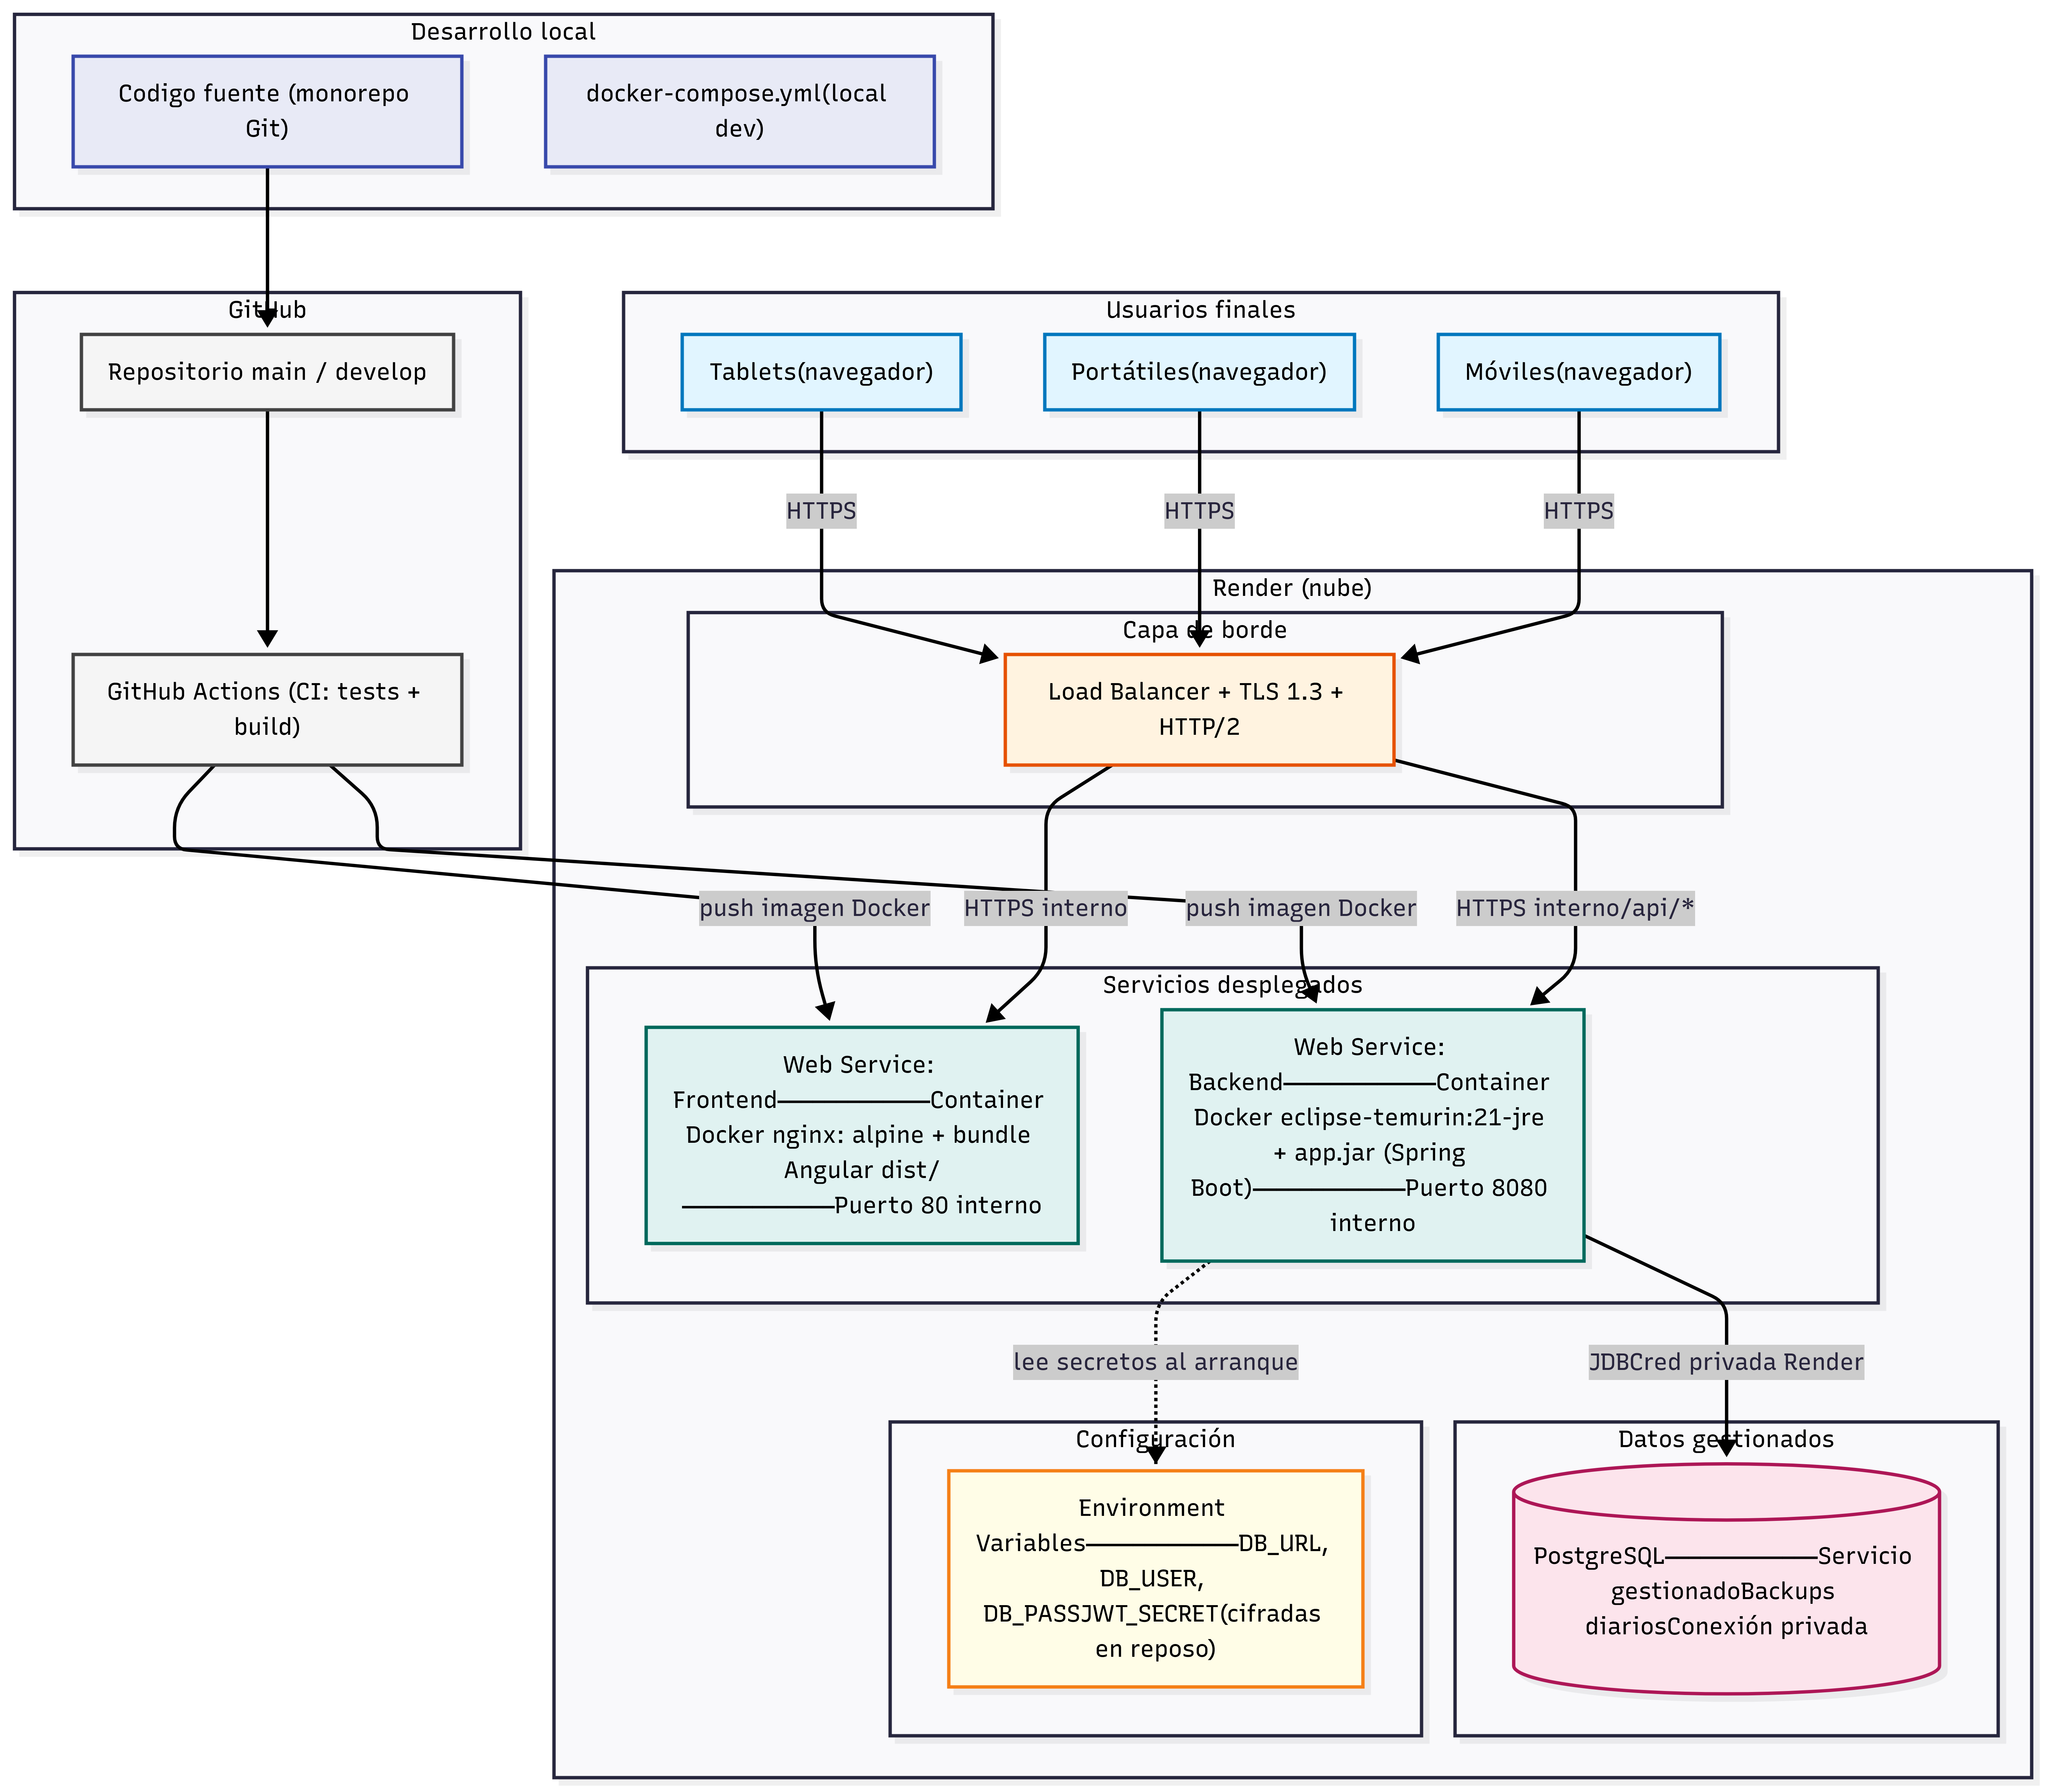
\includegraphics[width=1\linewidth]{assets/mermeid/Diagrama-despliegue-arquitectura.png}
\end{figure}
\par
\vspace{5mm}


\subsubsection{Entorno para la Implementación del Sistema Actual}
El sistema se implementará de forma local usando un proyecto en IntelliJ IDEA, con una base de datos 
PostgreSQL local (montada desde Docker) para desarrollo y pruebas. El entorno de desarrollo se configura mediante Docker Compose, 
que orquesta los contenedores de la aplicación y la base de datos, se harán commits a GitHub desde la misma
máquina donde el repositorio está configurado siguiendo estrategias CI en cada \texttt{pull request}, asi como enfoque tradicional de pruebas 
o TDD donde aplique para asegurar un sistema robusto en cada iteración. En Render se despliegue final cuando el stack backend y frontend haya sido 
previamente probado y optimizado en local. De esta manera, se aprovecha el periodo de 30 días de plan gratuito para someter el sistema completo 
a uso real y finalizar de optimizar lo necesario antes de tener que pagar mensualmente.

\newpage

\subsection{Suposiciones y Dependencias que Asume el Equipo en Torno al Proyecto}
\begin{itemize}
    \item El volumen de amigos atendidos se mantiene en el orden de magnitud
    actual (decenas, sin superar el centenar simultáneo) durante al menos
    los dos primeros años de operación del sistema.

    \item Los requisitos legales de la Ley 1/2025 no sufren modificaciones
    sustantivas durante el periodo de desarrollo. Si se publicaran
    reglamentos de desarrollo o instrucciones técnicas adicionales, sería
    necesario revisar el módulo de trazabilidad alimentaria.

    \item Además de la Ley 1/2025, no hay otras normativas sectoriales 
    (sanitarias, laborales, de protección de datos) que afecten directamente 
    a la operación del sistema. En caso de que se publicaran nuevas normativas, 
    sería necesario revisar el diseño del sistema para garantizar su cumplimiento integrándolo en él.
\end{itemize}


\subsubsection{Factores Externos que Tienen un Efecto en el Producto, pero No son Restricciones Obligatorias}
\begin{itemize}
    \item \textbf{Crecimiento de la asociación.} Si la asociación amplía su radio de
    acción geográfico o incorpora nuevas delegaciones, el modelo de datos
    necesitará incorporar el concepto de ``centro'' o ``delegación'' como
    entidad organizativa.
    
    \item \textbf{Incorporación de nuevas entidades donantes.} La incorporación de
    un nuevo donante con convenio formal podría implicar nuevas
    exigencias documentales, y el sistema no debería tener problemas para adaptarse.
    
    \item \textbf{Incremento en el precio sobre los planes de Render.} Si el coste de
    los planes contratados creciera por encima del nivel sostenible para
    la asociación, sería necesario evaluar la migración a un proveedor
    alternativo.
\end{itemize}


\subsection{Precios y Costes}
\subsubsection{Cómo se Estructura el Coste de Operación}
La operación del sistema se aloja en la plataforma Render, \textbf{cuyo modelo de
facturación se compone de tres conceptos sumables} que conviene conocer
para anticipar la evolución del gasto a lo largo del tiempo:
\begin{enumerate}
    \item \textbf{Plan del workspace}: una suscripción mensual fija que da derecho al
    uso de la plataforma y determina las funcionalidades disponibles
    (asientos de equipo, ventana de copias de seguridad, retención de
    logs, soporte). En 2026 Render eliminó las tarifas por usuario, de
    modo que el plan ya no se encarece al añadir voluntarios o miembros
    de la directiva con acceso al panel de administración.

    \item \textbf{Compute por servicio}: cada servicio desplegado (backend,
   frontend, base de datos) tiene su propio plan independiente, que
   determina la memoria, CPU y capacidades del servicio. Se factura
   al segundo, lo que significa que un servicio detenido
   no genera coste durante el tiempo que está parado.

   \item \textbf{Recursos métricos}: ancho de banda saliente, almacenamiento
   adicional de la base de datos, minutos de construcción del pipeline
   de despliegue. Solo se facturan si se exceden las cuotas incluidas
   en el plan del workspace.
\end{enumerate}

\subsubsection{Detalles Técnicos de las métricas de Render}
Detallamos conceptos técnicos relevantes para comprender el uso de Render y como afectan al coste:
\par
\vspace{5mm}
\textbf{¿Qué son los ``asientos de equipo''?} Asientos = personas con acceso al panel de administración de Render. 
Más allá del desarrollador principal, se puede conceder un \textit{asiento} a miembros de la coordinación o la directiva 
para que puedan monitorizar el estado del sistema, revisar logs o gestionar despliegues sin coste adicional.
\par
\vspace{5mm}
\textbf{¿Qué implica realmente cada métrica de compute?}
\begin{itemize}
    \item \textbf{Memoria (RAM):} la memoria viva donde el proceso (Spring Boot, PostgreSQL) guarda lo que está usando \textit{ahora} mismo.
    No depende del número de usuarios concurrentes, depende de lo que cada petición carga en memoria. Ejemplo, una petición que devuelve 100 
    amigos consume más RAM que una que devuelve 1.

    \item \textbf{CPU:} la potencia de cálculo. Ejemplo, una operación compleja (generar un PDF, ejecutar un mapeo 
    bancario sobre 1000 filas, calcular un informe agregado) consume mucha CPU.\ En cambio, devolver un registro consume poca CPU.\

    \item \textbf{Conexiones (solo en BD):} PostgreSQL atiende a cada cliente abriendo una conexión. Cada conexión consume RAM (aprox. 10 MB).
    En su uso, no debería tenerse más de máximo 10 conexiones simultáneas. 100 conexiones no son 100 usuarios concurrentes; son 100 
    conexiones simultáneas al servidor de BD.\

    \item \textbf{Bandwidth:} datos que salen de Render hacia los navegadores de los usuarios. Para el volumen de 
    accesos que vamos a tener no son un factor determinante.

    \item \textbf{build minutes:} el tiempo de CPU consumido cada vez que Render compila tu app para desplegarla. 
    Para controlarlo, no hacer deploys triviales (ejemplo, cada vez que haces un commit a la rama de producción) 
    sino solo cuando hay cambios significativos que justifiquen el despliegue de una nueva versión.
\end{itemize}

\subsubsection*{Como monitorizar en general}
Render te ofrece gráficas integradas en el dashboard que ayudan a visualizar el consumo de cada métrica en tiempo real 
y a lo largo del tiempo. Es recomendable revisar estas gráficas semanalmente para detectar patrones de 
uso, picos inesperados o tendencias que puedan indicar la necesidad de ajustar la configuración 
(ejemplo, aumentar RAM si se detectan picos frecuentes de memoria).

\begin{figure}[H]
    \centering
    \caption{Ejemplo de métricas en el dashboard de Render}
    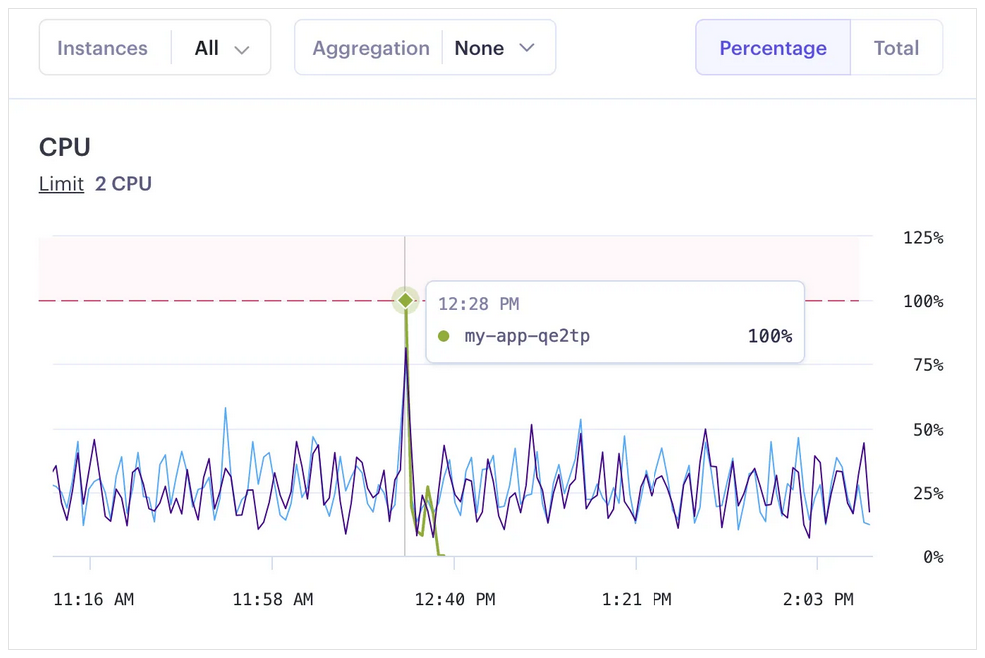
\includegraphics[width=0.50\linewidth]{assets/Ejemplo-metricas-Render1.png}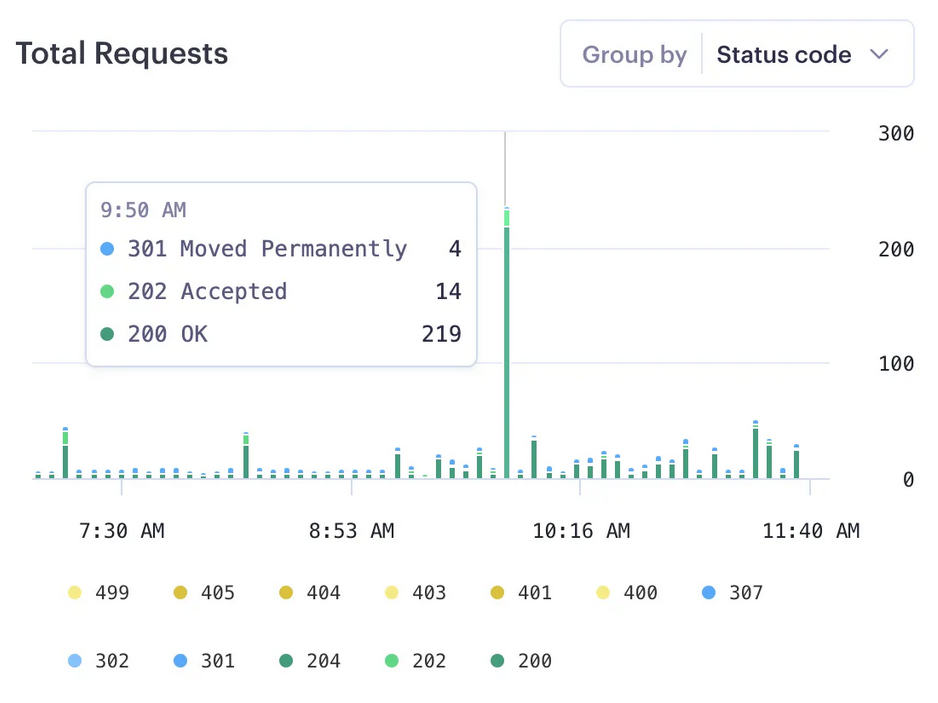
\includegraphics[width=0.50\linewidth]{assets/Ejemplo-metricas-Render2.png}
    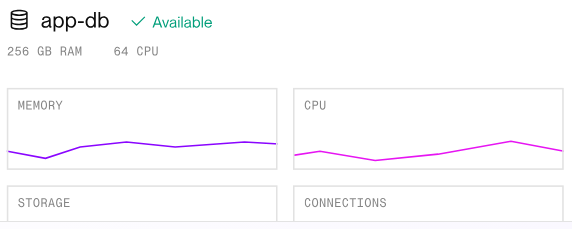
\includegraphics[width=0.50\linewidth]{assets/Ejemplo-metricas-Render3.png}
\end{figure}
\par
\vspace{5mm}

\subsubsection{Estimación de Coste para la Configuración Inicial}
A continuación se presenta la estimación de coste mensual para la
configuración con la que el sistema entrará en operación. Las cifras
están expresadas en dólares estadounidenses (USD), unidad de
facturación de Render, y se han verificado contra la tarifa pública del
proveedor en mayo de 2026.

\vspace{5mm}

\begin{longtable}[]{@{}
    % Metadatos de la tabla
        p{0.23\columnwidth}
        p{0.22\columnwidth}
        p{0.22\columnwidth}
        p{0.22\columnwidth}@{}}

    \caption{Coste para la Configuración Inicial} \\

    % Configuración de la tabla para repetir encabezados en cada página
    \toprule
    \textbf{Concepto} & \textbf{Plan} & \textbf{Características} & \textbf{Coste mensual} \\
    \midrule
    \endfirsthead % chktex 1

    \toprule
    \textbf{Concepto} & \textbf{Plan} & \textbf{Características} & \textbf{Coste mensual} \\
    \midrule
    \endhead % chktex 1

    \midrule
    \multicolumn{2}{r}{\small\emph{Continúa en la siguiente página}} \\
    \endfoot % chktex 1

    \bottomrule
    \endlastfoot % chktex 1

    % Cuerpo de la tabla
    Plan del workspace & Hobby & Gratuito, hasta 25 servicios, 5 GB de bandwidth, 
    copias de seguridad de 3 días & 0 USD \\
    \midrule

    Backend (Spring Boot) & Starter & 512 MB RAM, 0.5 CPU, sin hibernación & 7 USD \\
    \midrule

    Frontend (Angular) & Static Site & Servido desde CDN global, TLS automático & 0 USD \\
    \midrule

    Base de datos & PostgreSQL Basic-256mb & 256 MB RAM, 1 GB almacenamiento, 100 conexiones & 6 USD \\
    \midrule

    Dominio propio (.org / .es) & Anualidad prorrateada & Registro a través de proveedor externo & aprox. 1 USD \\ % chktex 26
    \midrule

    \textbf{Total estimado:} & & & \textbf{aprox. 14 USD/mes} \\
\end{longtable}

Considerar que dependiendo de la entidad bancaria, al momento de hacer\textbf{ el pago se puede cobrar una comisión por cambio 
de divisa}, lo que incrementaría el coste mensual.

\par
\vspace{5mm}

Este coste equivale aproximadamente a entre 13 y 15 EUR mensuales según
el tipo de cambio vigente. Es la configuración más eficiente compatible
con un funcionamiento continuo de producción, sin tiempos de espera al
acceder al sistema y con copias de seguridad automáticas de la base de
datos.


\subsubsection{Evolución Prevista del Coste}
A medida que el sistema gana adopción y la asociación afina su uso, el
coste mensual puede aumentar. La progresión razonable
prevista es la siguiente: meses 1 a 6 (desarrollo + primer período de uso) con el costo inicial (tabla anterior).
\par
\vspace{5mm} 
Luego ver como evoluciona en los meses 7 a 18 (operación con todo el voluntariado) para considerar migración del workspace 
al plan Pro con una base de datos a un nivel superior si hiciera falta (hasta 52 USD/mes). 
\par
\vspace{5mm}
Finalmente, a partir del año 2, 
si el uso se mantiene o crece, considerar ampliación de capacidad del backend (hasta 70 USD/mes) o limpieza de servicios 
no utilizados para optimizar costes o cambio de proveedor si el coste se vuelve insostenible.


\subsubsection{Modelo Económico del Producto}
El sistema es un desarrollo a medida sin modelo comercial asociado.
No se contempla su venta ni su licenciamiento a terceros en la versión
inicial. Si en el futuro otras asociaciones similares manifestaran
interés, podría evaluarse la liberación del código bajo licencia de
software libre o un modelo de servicio gestionado, pero esta decisión
queda fuera del alcance del presente documento.


\subsection{Estrategia de Mantenimiento}
Al ser una aplicación web, el usuario final no instala nada en su
dispositivo. El acceso al sistema se realiza mediante la dirección web
proporcionada por la asociación, abierta en el navegador de su
dispositivo al sitio web desplegado por Render.
\par
\vspace{5mm}
Las responsabilidades de despliegue y mantenimiento se
distribuyen como sigue:

\subsubsection*{Render asume:}
\begin{itemize}
    \item Provisión de la infraestructura física subyacente (servidores,
    almacenamiento, red).

    \item Mantenimiento del sistema operativo subyacente y parches de 
    seguridad de plataforma.

    \item Provisión y mantenimiento del servicio gestionado de PostgreSQL, 
    incluidas copias de seguridad diarias.

    \item Renovación automática del certificado TLS.\

    \item Monitorización de la salud básica del servicio (uptime, métricas de plataforma).

    \item Cifrado de las variables de entorno en reposo.
\end{itemize}


\subsubsection*{El equipo de desarrollo asume:}
\begin{itemize}
    \item Construcción y mantenimiento de las imágenes Docker.
    
    \item Configuración de los servicios en Render (variables de entorno,
    conexiones, escalado).

    \item Mantenimiento del pipeline de integración y despliegue continuos.
    
    \item Aplicación de actualizaciones de seguridad a las dependencias del proyecto.
    
    \item Implementación de copias de seguridad propias adicionales como redundancia.
    
    \item Monitorización aplicativa (logs, errores, métricas de negocio).
    
    \item Soporte funcional al usuario final.
\end{itemize}
\section{Requisitos Funcionales}
Este capítulo describe de forma estructurada \textbf{las acciones que el sistema debe
ser capaz de realizar} para cumplir los objetivos establecidos en los capítulos
anteriores. 
\par
\vspace{4mm}
Cuando un requisito tiene reglas de negocio asociadas o
condiciones de error que merecen detalle, estas se listan bajo
la descripción principal.

\subsection{RF1 Gestión de Cuentas y Autenticación}
\begin{itemize}
    \item \textbf{RF1.1 Creación de cuentas de voluntario} \\
    El sistema debe permitir al usuario con rol Admin o voluntario con rol adecuado crear nuevas cuentas de voluntario en el sistema. 
    Los datos que se registran en el formulario son:
    \begin{description}
        \item[-] Nombre.
        \item[-] Apellidos.
        \item[-] Teléfono.
        \item[-] DNI. % chktex 13
        \item[-] Correo electrónico.
        \item[-] Rol.
        \item[-] Nivel de seguridad.
        \item[-] Area profesional del voluntario. 
        \item[-] Capacidades en el sistema.
    \end{description}
    \par
    Adicionalmente, el sistema registrará automáticamente la siguiente información de la cuenta en todo momento:
    \begin{description}
        \item[-] Estado de la cuenta.
        \item[-] Contraseña encriptada.
        \item[-] Fecha de creación de la cuenta al finalizar la creación.
        \item[-] Fecha del último login del voluntario.
        \item[-] Intentos fallidos al intentar iniciar sesión de forma incorrecta.
        \item[-] Fecha hasta donde se bloquea la cuenta tras 5 intentos fallidos al iniciar sesión. 
    \end{description}
    \par
    La creación de una nueva cuenta queda registrada en el log de auditoría con el nombre de la cuenta actualmente autenticada en el sistema. 
    \par
    El admin proporciona al voluntario una contraseña de un solo uso para entrar al sistema. Una vez inicie el voluntario, se le pedirá que introduzca 
    su nueva contraseña ed acceso para sustituir la temporal proporcionada. En este momento, el estado de la cuenta se actualiza de \texttt{PENDIENTE\_ACTIVACION} a 
    \texttt{ACTIVA} (RF1.8).
    
    \item \textbf{RF1.2 Visualización de los datos de la cuenta} \\
    El sistema debe permitir a cualquier voluntario autenticado consultar los
    datos de su propia cuenta.

    \item \textbf{RF1.3 Edición de los datos de la cuenta} \\
    El sistema debe permitir a cualquier voluntario autenticado modificar los
    datos personales de su propia cuenta.

    \item \textbf{RF1.4 Eliminación de cuentas} \\
    El sistema debe permitir al Admin eliminar definitivamente una cuenta de
    voluntario sólo si esta no tiene operaciones históricas asociadas.
    \begin{description}
        \item[-] Si la cuenta tiene operaciones registradas, la eliminación se rechaza
        y se ofrece la alternativa de desactivación (RF1.5).
        \item[-] La eliminación deja constancia en el log de auditoría con el
        identificador y nombre de la cuenta eliminada.
    \end{description}

    \item \textbf{RF1.5 Desactivación de cuentas} \\
    El sistema debe permitir al Admin desactivar la cuenta de un voluntario sin eliminarla del sistema.
    \begin{description}
        \item[-] La desactivación es reversible por el Admin en cualquier momento.
        \item[-] Una cuenta desactivada no permite inicio de sesión.
    \end{description}

    \item \textbf{RF1.6 Inicio de sesión} \\
    El sistema debe permitir a un voluntario iniciar sesión introduciendo su
    correo electrónico y contraseña.
    \begin{description}
        \item[-] Tras un inicio de sesión correcto, el sistema emite un token JWT con
        validez limitada que el cliente almacena en memoria del SPA.\@
        \item[-] Los intentos fallidos quedan registrados en el log de auditoría. Varios intentos fallidos 
        consecutivos provoca un bloqueo temporal el inicio de sesión.
    \end{description}

    \item \textbf{RF1.7 Cierre de sesión} \\
    El sistema debe permitir a un voluntario cerrar sesión de forma explícita invalidando el token JWT 
    del lado del cliente.
    \begin{description}
        \item[-] El sistema debe ofrecer cierre de sesión automático tras un periodo
        configurable de inactividad.
    \end{description}

    \item \textbf{RF1.8 Activación de la cuentas} \\
    El sistema debe permitir a un voluntario activar su cuenta actualizando la contraseña temporal de acceso por una nueva que introduzca. 
    El estado de cuenta debe ser \texttt{ACTIVA} tras esta acción.
\end{itemize}




\subsection{RF2 Control de Acceso y Roles}
\begin{itemize}
    \item \textbf{RF2.1 Roles del sistema} \\
    El sistema debe implementar los cinco roles definidos en la sección 4.3, cada uno
    con su matriz de permisos por defecto: \texttt{ADMIN}, \texttt{OPERATIVO},
    \texttt{PROFESIONAL}, \texttt{PUENTE} y \texttt{AGENTE\_TEMP}.

    \item \textbf{RF2.2 Asignación de funciones específicas} \\
    El sistema debe permitir al Admin asignar a un voluntario, además de su
    rol, un conjunto de funciones específicas que limiten o amplíen los
    permisos por defecto del rol.
    \begin{description}
        \item[-] Las funciones específicas no pueden otorgar a un voluntario
        capacidades que su rol no le permita por diseño (un \texttt{OPERATIVO} no
        puede recibir la capacidad \texttt{IMPORTAR\_EXTRACTOS}, exclusiva del Admin).
    \end{description}

    \item \textbf{RF2.3 Niveles de visibilidad de datos sensibles} \\
    El sistema debe asignar a cada voluntario uno de los niveles de
    seguridad descritos en la sección 4.3: \texttt{BASICO} o \texttt{PRIVILEGIADO}.
    \begin{description}
        \item[-] El nivel \texttt{BASICO} ve únicamente los datos no sensibles de la ficha del amigo y
        los servicios prestados a él más no el motivo o notas que justifiquen esos servicios.
        \item[-] El nivel \texttt{PRIVILEGIADO} ve todos los datos. El Admin tiene siempre nivel y puede otorgarlo a otros voluntarios.
    \end{description}

    \item \textbf{RF2.4 Habilitación temporal de acceso} \\
    El sistema debe permitir al Admin habilitar a un voluntario profesional
    acceso de lectura a los datos sensibles de un amigo concreto durante una
    ventana de tiempo limitada.
    \begin{description}
        \item[-] La habilitación se asocia al par voluntario-amigo y a una fecha de
        caducidad. Alcanzada la fecha de caducidad, el acceso se revoca automáticamente sin intervención manual.
        \item[-] Toda actividad realizada bajo una habilitación temporal queda
        registrada en el log de auditoría con marcado especial.
    \end{description}
    
    \item \textbf{RF2.5 Revocación de habilitaciones temporales} \\
    El sistema debe permitir al Admin revocar una habilitación temporal antes
    de su caducidad.
    \begin{description}
        \item[-] La revocación es inmediata: la siguiente petición del voluntario
        afectado falla con código de autorización denegada.
        \item[-] La revocación queda registrada en el log de auditoría.
    \end{description}
    
    % FIXME: No se interpretar este requisito. ¿Qué es exactamente la "verificación de autorización en backend"?
    \item \textbf{RF2.6 Verificación de autorización en backend} \\
    El sistema debe verificar las reglas de autorización en el lado del
    servidor para toda operación que acceda a datos sensibles o que
    modifique el estado del sistema.
\end{itemize}




\subsection{RF3 Gestión de Amigo}
\begin{itemize}
    \item \textbf{RF3.1 Creación de ficha mínima} \\
    El sistema debe permitir crear una ficha de amigo introduciendo
    únicamente nombre.
    \begin{description}
        \item[-] El cambio de nivel queda registrado en el log de auditoría con 
        identificador del voluntario que lo realiza y timestamp.
        \item[-] La creación de la ficha queda registrada en el log de auditoría.
        \item[-] Se registra la fecha de creación en su ficha. 
    \end{description}
    \begin{itemize}
        \item \textbf{RF3.1.1 Registro de entrega objetos} \\
        En cualquier nivel de confianza (RF3.2) está disponible una caja de texto donde se registran objetos o pertenencias 
        del amigo al momento de entrar en el centro. Si son más de uno deben separarse por comas (, ) para que el sistema los procese % chktex 37
        correctamente y se muestren en la ficha del amigo en forma de listado de checkboxes. Caso paradigmático: amigo entrega pasaporte/DNI para que se guarde en la caja 
        fuerte del centro. En su lugar, se les otorga una copia.
        \begin{description}
            \item[-] El texto escrito aparecerá en la ficha correspondiente del amigo (RF3.4). Puede dejarse en blanco.
        \end{description}
        \item \textbf{RF3.1.2 Registro de devolución de objetos} \\
        El sistema registra en el log de auditoría la devolución de un objeto a un amigo con el nombre del usuario actualmente autenticado que realizó la devolución. Se actualiza consecuentemente su ficha de amigo 
        para reflejar que el objeto ya no está en posesión del centro. Caso paradigmático: se devuelve el DNI original al amigo para realizar un trámite legal.
    \end{itemize}

    \item \textbf{RF3.2 Escalado del nivel de confianza}
    \begin{itemize}
        \item \textbf{RF3.2.1 Nivel 1 $-$ Anónimo} \\
        Estado inicial. Campos disponibles: nombre y, opcionalmente, una descripción corta.
        \item \textbf{RF3.2.2 Nivel 2 $-$ Frecuente} \\
        Tras varias visitas o cuando la coordinación lo decida. Habilita los
        campos como pueden ser: apellidos, fecha de nacimiento, género, tallas (ropa y
        calzado), idioma principal, teléfono.
        \item \textbf{RF3.2.3 Nivel 3 $-$ Entrevistado} \\
        Tras una entrevista de profundidad. Habilita los campos: DNI o
        documento equivalente (NIE, pasaporte), nacionalidad, dirección, datos
        sensibles (situación administrativa, médica, psicológica, jurídica),
        notas privadas.
    \end{itemize}
    
    \item \textbf{RF3.3 Edición de ficha} \\
    El sistema debe permitir editar los campos disponibles en el nivel actual de la ficha.
    \begin{description}
        \item[-] Cada modificación queda registrada en el log de auditoría con valor 
        anterior, valor nuevo, voluntario y marca de tiempo.
        \item[-] Todos los campos son editables por el Admin o voluntariado con permisos adecuados.
    \end{description}
    
    \item \textbf{RF3.4 Visualización de ficha} \\
    El sistema debe permitir visualizar la ficha de un amigo aplicando las
    reglas de visibilidad por nivel de seguridad descritas en RF2.3.
    
    \item \textbf{RF3.5 Búsqueda y listado de amigos} \\
    El sistema debe permitir buscar y listar amigos aplicando filtros por
    nombre, alias, nivel de confianza y fecha de última visita mostrando información acorde a
    el nivel de seguridad del voluntario que consulta.
    
    
    \item \textbf{RF3.6 Histórico individual del amigo}\hypertarget{RF3.6}{} \\
    El sistema debe mantener y mostrar para cada amigo el histórico
    completo de su relación con la asociación:
    \begin{description}
        \item[-] Servicios solicitados, agendados y prestados (con fecha, voluntario, observaciones).
        \item[-] Entregas materiales recibidas (prenda, talla, fecha, voluntario).
        \item[-] Operaciones de lavandería (entrada de prenda propia, devolución).
        \item[-] Entradas y salidas alimentarias asociadas (cuando aplique).
        \item[-] Gastos vinculados al amigo (RF7.6).
        \item[-] Comunicaciones externas registradas (RF3.8).
        \item[-] Cambios de nivel de confianza con fechas y motivos.
    \end{description}

    \item \textbf{RF3.7 Registro de tallas} \\
    El sistema debe almacenar las tallas de ropa y calzado del amigo.
    
    \item \textbf{RF3.8 Trazabilidad de comunicaciones externas} \\
    El sistema debe permitir registrar manualmente comunicaciones externas
    realizadas en nombre del amigo o relacionadas con su expediente, con el
    fin de mantener un historial consolidado.
    \begin{description}
        \item[-] Tipos de comunicación: correo electrónico, llamada telefónica, gestión presencial, documento enviado o recibido.
        \item[-] Cada comunicación se registra con: tipo, contraparte (entidad o persona externa), fecha, asunto y notas opcionales.
    \end{description}

    \item \textbf{RF3.9 Notas privadas} \\
    El sistema debe permitir asociar notas privadas a la ficha de un amigo. Son
    visibles únicamente para voluntarios con nivel de seguridad \texttt{PRIVILEGIADO} o
    con habilitación temporal vigente al área correspondiente más cualquier voluntario puede añadir notas. 
    Caso paradigmático: un amigo le cuenta su historia por partes a diferentes voluntarios (con los que más simpatiza será más honesto). Registran esas notas puntuales. 
    Al cabo de varias notas se puede armar una linea temporal completa de la vida del amigo.
    \begin{description}
        \item[-] Las notas son inmutables una vez guardadas: no se editan, sino que se
        añaden notas adicionales que matizan o corrigen las previas.
        \item[-] Cada nota lleva identificador del voluntario autor y un timestamp de creación.
    \end{description}
\end{itemize}




\subsection{RF4 Servicios y Agendamiento}
\begin{itemize}
    \item \textbf{RF4.1 Gestión del Catálogo de servicios} \\
    El sistema debe mantener un catálogo de tipos de servicio que el Admin
    puede consultar y eliminar o desactivar algún según sea el caso.
    \begin{description}
        \item[-] La eliminación de un tipo de servicio queda condicionada a la ausencia
        de servicios prestados de ese tipo en el histórico (en su lugar, se
        desactiva).
    \end{description}

    \item \textbf{RF4.2 Agendamiento de un servicio} \\
    El sistema debe permitir agendar la prestación de un servicio a un amigo en una fecha y franja horaria concretas.
    \begin{description}
        \item[-] El sistema verifica al agendar que no se excede la capacidad del turno (RF4.3).
    \end{description}

    \item \textbf{RF4.3 Control de capacidad por turno} \\
    El sistema debe impedir el agendamiento de un servicio que excedería la
    capacidad máxima del turno correspondiente.
    
    \item \textbf{RF4.4 Regla de prerrequisito de agendamiento} \\
    El sistema debe impedir el registro de prestación de un servicio si no existe un agendamiento previo asociado.
    \begin{description}
        \item[-] La ducha es el caso paradigmático: sin agendamiento previo no se presta el servicio aunque haya espacio disponible.
    \end{description}
    
    \item \textbf{RF4.5 Registro de prestación de servicio efectiva} \\
    El sistema debe permitir al voluntario registrar la prestación efectiva
    del servicio en el momento o tras producirse.
    \begin{description}
        \item[-] Resultado posibles: prestado, no prestado por ausencia del amigo, no
        prestado por ausencia del voluntario, cancelado por la coordinación.
        \item[-] En caso de prestación, se registran observaciones opcionales del motivo de prestación del servicio 
        sólo visible para voluntarios autorizados.
        \item[-] La prestación queda asociada al amigo y aparece en su histórico (RF3.6).
    \end{description}
    
    \item \textbf{RF4.6 Visualización de la agenda} \\
    El sistema debe permitir visualizar la agenda del centro en formato calendario diario, semanal y mensual.
    \begin{description}
        \item[-] Cada agendamiento se muestra con tipo de servicio, amigo asociado y voluntario responsable.
        \item[-] La vista diaria es accesible directamente desde la pantalla principal.
        \item[-] Filtros disponibles: por tipo de servicio, por voluntario, por amigo.
    \end{description}
    
    \item \textbf{RF4.7 Reagendamiento y cancelación} \\
    El sistema debe permitir modificar la fecha, franja o voluntario asignado de un agendamiento, así como cancelarlo.
    \begin{description}
        \item[-] Cualquier modificación queda registrada en el log de auditoría.
        \item[-] La cancelación no elimina el registro: lo marca como cancelado con motivo opcional y voluntario que cancela.
    \end{description}
\end{itemize}




\subsection{RF5 Inventario, Entregas y Lavandería}
\begin{itemize}
    \item \textbf{RF5.1 Cuaderno de Entradas y Salidas} \\
    El sistema debe mantener un inventario del stock disponible en el
    armario general, organizado por tipo de prenda y talla.
    \begin{description}
        \item[-] El sistema muestra el inventario en una vista de cuadrícula que
        permite filtrar por tipo y talla. 
    \end{description}

    \item \textbf{RF5.2 Registro de entrada de stock} \\
    El sistema debe permitir registrar la entrada de prendas donadas al
    armario general.
    \begin{description}
        \item[-] La entrada incrementa automáticamente el stock correspondiente.
        \item[-] Es posible registrar varias prendas en una misma operación (entrada por lotes). 
    \end{description}

    \item \textbf{RF5.3 Registro de entrega de prenda} \\
    El sistema debe permitir registrar la entrega de una prenda concreta a un amigo.
    
    \begin{itemize}
        \item \textbf{RF5.3.1 Decremento automático de stock} \\
        La entrega decrementa automáticamente la cantidad disponible de la
        combinación tipo-talla entregada en una unidad.
        \item \textbf{RF5.3.2 Reglas de frecuencia configurables} \\
        El sistema debe aplicar reglas de frecuencia configurables que limiten
        la entrega repetida del mismo tipo de prenda al mismo amigo en un
        periodo dado.
        \begin{description}
            \item[-] Caso paradigmático: una unidad de calzado por amigo cada 3 meses.
            \item[-] Si la regla se incumple, el sistema avisa al voluntario y exige justificación o aprobación de un Admin.
            \item[-] Las excepciones quedan registradas en el log de auditoría. 
        \end{description}
        \item \textbf{RF5.3.3 Integridad ante stock insuficiente} \\
        El sistema debe impedir la entrega de una prenda cuya cantidad disponible es cero. 
        Ni siquiera debe mostrarse como opción seleccionable en el proceso de entrega.
    \end{itemize}

    \item \textbf{RF5.4 Alertas de reposición} \\
    El sistema debe permitir definir, por combinación tipo-talla, un umbral
    mínimo de stock por debajo del cual se genera una alerta visual en el
    panel del armario.

    \item \textbf{RF5.5 Visualización del histórico de lavandería} \\
    El sistema debe ofrecer una vista del histórico de lavandería tanto a
    nivel global del centro (todas las prendas en proceso) como a nivel
    individual del amigo.
    \begin{description}
        \item[-] El histórico individual aparece en la ficha del amigo (RF3.6).
        \item[-] El histórico global es accesible desde el módulo de inventario.
    \end{description}
\end{itemize}




\subsection{RF6 Trazabilidad Alimentaria (Cumplimiento Ley 1/2025)}
\begin{itemize}
    \item \textbf{RF6.1 Registro de entrada de alimento} \\
    El sistema debe permitir registrar la entrada de alimentos al centro,
    con todos los datos necesarios para satisfacer las exigencias de
    trazabilidad de la Ley 1/2025.
    \begin{itemize}
        \item \textbf{RF6.1.1 Origen del alimento} \\
        Cada entrada debe categorizarse según su origen:
        \begin{description}
            \item[-] Compra propia: realizada por la asociación. Requiere ticket de compra asociado.
            % \item[-] Donación de entidad con convenio: requiere convenio activo registrado (RF6.x) y, cuando proceda, albarán de entrega. % No se incluye en esta fase 
            \item[-] Donación de entidad sin convenio: para donaciones puntuales de entidades sin acuerdo formal.
            \item[-] Donación particular: Persona que aporta espontáneamente. En este caso, el ticket suele no estar disponible y debe quedar documentado el motivo.
        \end{description}
        \par 
        Todo ticket o albarán recibido debe almacenarse físicamente y estar disponible para auditoría.
        \item \textbf{RF6.1.2 Datos obligatorios de la entrada} \\
        Independientemente del origen, toda entrada registra: 
        \begin{description}
            \item[-] Tipo de producto.
            \item[-] Categoría general (lácteos, panadería, fruta\ldots)
            \item[-] Cantidad y unidad (kilos, litros, unidades).
            \item[-] Fecha de entrada.
            \item[-] Voluntario que registra.
            \item[-] Lugar de almacenamiento (despensa, congelador\ldots)
        \end{description}
        \item \textbf{RF6.1.3 Datos específicos de seguridad alimentaria} \\
        Para todo producto perecedero o susceptible de control sanitario:
        \begin{description}
            \item[-] Lote del fabricante, cuando esté disponible.
            \item[-] Fecha de caducidad o consumo preferente.
            \item[-] Para productos refrigerados: temperatura de recepción.
            \item[-] Check\footnote{Se refiere a una verificación física, y se marca con un \textit{check} que el estado del producto es aceptable.} de verificación de higiene y estado del producto al recibirse.
            \item[-] Lugar y método de almacenamiento.
        \end{description}
    \end{itemize}

    \item \textbf{RF6.2 Registro de salida de alimento} \\
    El sistema debe permitir registrar la salida de alimento del stock
    hacia su consumo o destino final.
    \begin{description}
        \item[-] Cada salida incluye: producto, cantidad, fecha, turno (mañana o tarde), tipo de salida y voluntario que registra.
        \item[-] Tipos de salida: desayuno, merienda, cena, café, comida individual a un amigo, retirada por caducidad, retirada por deterioro.
        \item[-] La salida decrementa automáticamente el stock disponible.
        \item[-] Se registra el voluntario que realizo la salida.
    \end{description}

    \item \textbf{RF6.3 Clasificación por prioridad legal} \\
    Toda entrada y, cuando aplique, toda salida del sistema deben
    clasificarse según las cuatro categorías de prioridad de aprovechamiento
    establecidas por la Ley 1/2025:
    \begin{description}
        \item[-] Prioridad 1: Consumo humano. Categoría por defecto.
        \item[-] Prioridad 2: Alimentación animal.
        \item[-] Prioridad 3: Subproducto (compostaje, biocombustible).
        \item[-] Prioridad 4: Residuo.
        \item[-] Toda salida con prioridad distinta de 1 requiere justificación
        obligatoria: motivo (caducidad, deterioro, rechazo, otros) y
        observaciones.
        \item[-] El sistema mantiene un contador agregado por prioridad para los informes legales.
    \end{description}

    \item \textbf{RF6.4 Control de stock alimentario} \\
    El sistema debe mantener una vista de stock alimentario actual
    diferenciada del armario general (RF5.1), con visibilidad de:
    \begin{description}
        \item[-] Cantidad disponible por tipo de producto.
        \item[-] Lotes activos con sus fechas de caducidad.
        \item[-] Productos próximos a caducar (umbral configurable por defecto a 7 días).
        \item[-] Productos caducados pendientes de retirada.
    \end{description}

    % \item \textbf{RF6.5 Asociación de salida a amigo} \\
    % El sistema debe permitir, opcionalmente, asociar una salida concreta a un amigo identificado.
    % \begin{description}
    %     \item[-] Esta asociación puede incrementar la carga de trabajo de los voluntarios en el día a día. Sin embargo, se 
    %     considera que refuerza la trazabilidad y permite generar
    %     informes de consumo individualizado (por ejemplo, \textit{``café tomado por
    %     Marcos durante el último semestre''}).
    %     \item[-] La asociación, cuando se usa, aparece en el histórico del amigo (RF3.6). 
    % \end{description}

    \item \textbf{RF6.5 Generación del cuaderno de trazabilidad} \\
    El sistema debe generar el cuaderno completo de entradas y
    salidas alimentarias en un periodo definido, en formato apto para
    inspección sanitaria.
    \begin{description}
        \item[-] Formatos aptos: PDF (impresión) y CSV (análisis).
        \item[-] Contenido: todas las entradas con sus datos completos (RF6.1), todas
        las salidas (RF6.2), todos los productos retirados con justificación
        (RF6.3) y saldo de stock al cierre del periodo.
        \item[-] El cuaderno generado para un periodo cerrado debe ser inmutable: no
        puede regenerarse con datos modificados a posteriori sin que quede
        constancia de la modificación.
    \end{description}

    \item \textbf{RF6.6 Inmutabilidad de registros cerrados} \\
    El sistema debe impedir la modificación o eliminación de registros de
    entrada o salida con antigüedad superior a un umbral configurable (por
    defecto, 30 días).
    \begin{description}
        \item[-] Esta regla protege la integridad documental del cuaderno frente a inspecciones.
        \item[-] Si una corrección es necesaria tras el cierre, se realiza mediante asientos
        compensatorios (entrada o salida correctiva con motivo \texttt{Rectificación}), no mediante edición del registro original.
    \end{description}
\end{itemize}

\subsection*{RF7 Gestión Financiera y Trazabilidad de Gasto}
\begin{itemize}
    \item \textbf{RF7.1 Catálogo de cuentas bancarias y caja} \\
    El sistema debe permitir registrar y mantener las cuentas a través de
    las cuales la asociación gestiona sus movimientos.
    \begin{description}
        \item[-] Para cada cuenta bancaria: nombre, entidad, número de cuenta 
        parcialmente enmascarado, tipo (corriente, caja chica, otra), estado (activa, inactiva).
        \item[-] La caja chica se modela como una cuenta de tipo efectivo.
        \item[-] Una cuenta no puede eliminarse si tiene asientos asociados; en su lugar, se desactiva. 
    \end{description}

    \item \textbf{RF7.2 Catálogo de categorías de gasto e ingreso} \\
    El sistema debe mantener un catálogo de categorías funcionales que el
    Admin puede ampliar y modificar.
    \begin{description}
        \item[-] El catálogo inicial reproduce las categorías que la asociación utiliza actualmente. Ejemplos: Suministros $-$ Agua/Luz, Gastos
        bancarios, Donaciones recibidas, Tasas de DNI, Medicamentos, productos de higiene, etc.
        \item[-] La eliminación de una categoría queda condicionada a la ausencia de asientos asociados; en su lugar, se desactiva.
    \end{description}

    \item \textbf{RF7.3 Catálogo de cuentas contables} \\
    El sistema debe permitir mantener, opcionalmente, un catálogo de
    códigos de cuenta contable conformes al criterio que la gestoría
    utiliza con la asociación.
\begin{description}
    \item[-] Cada cuenta contable incluye: código (por ejemplo ``6280'') y nombre descriptivo (por ejemplo ``Suministros $-$ Agua'').
    \item[-] El uso de cuenta contable en cada asiento es opcional: si la contabilidad llevada por la directiva no lo requiere, este catálogo puede permanecer vacío.
\end{description}

    \item \textbf{RF7.4 Registro manual de asientos contables} \\
    El sistema debe ofrecer un formulario para registrar manualmente cada
    asiento contable, reproduciendo digitalmente el flujo que la
    contabilidad de la asociación lleva hoy en Excel.
    \begin{itemize}
        \item \textbf{RF7.4.1 Campos del asiento} \\
        \begin{description}
            \item[-] \texttt{Fecha:} fecha del movimiento. Obligatorio.
            \item[-] \texttt{Concepto}: descripción libre del movimiento. Obligatorio.
            \item[-] \texttt{Cuenta bancaria}: cuenta o caja a la que se carga o abona el movimiento (RF7.1). Obligatorio.
            \item[-] \texttt{Cuenta contable}: código contable asociado (RF7.3). Opcional.
            \item[-] \texttt{Categoría}: clasificación funcional del movimiento (RF7.2). Obligatorio.
            \item[-] \texttt{Importe}: cantidad en euros, con signo (negativo para gasto, positivo para ingreso). Obligatorio.
            \item[-] \texttt{Tipo de gasto}: Casa, Amigo o Mixto (RF7.4.4). Obligatorio para gastos; no aplica a ingresos. 
            \item[-] \texttt{Amigo vinculado}: ficha del amigo asociado al gasto, sólo habilitado si el tipo es Amigo o Mixto. Opcional pero recomendado.
            \item[-] \texttt{Servicio vinculado}: servicio del catálogo (RF4.1) al que se asocia el gasto. Opcional.
            \item[-] \texttt{Referencia al archivo físico}: texto libre donde el usuario puede anotar la ubicación del justificante físico (``Carpeta abril 2026, ticket 7''). Opcional.
        \end{description}
        \item \textbf{RF7.4.2 Validación de los datos} \\
        El sistema debe validar al envío del formulario:
        \begin{description}
            \item[-] Los campos obligatorios están cumplimentados.
            \item[-] El importe es un número con dos decimales máximo.
            \item[-] Las cuentas y categorías referenciadas existen y están activas.
        \end{description}
        \item \textbf{RF7.4.3 Persistencia y auditoría} \\
        Cada asiento creado queda registrado con:
        \begin{description}
            \item[-] Identificador interno único e inmutable.
            \item[-] Marca de tiempo de creación.
            \item[-] Voluntario que lo registró.
            \item[-] Las modificaciones posteriores quedan registradas en el log de
            auditoría con valor anterior, valor nuevo, voluntario y marca de
            tiempo (RNF de auditoría).
        \end{description}
        \item \textbf{RF7.4.4 Categorización del gasto por destinatario} \\
        Cada gasto se clasifica obligatoriamente en una de tres categorías de destinatario:
        \begin{description}
            \item[-] \texttt{Casa}: gasto puro de la asociación (suministros generales, servicios, insumos comunes).
            \item[-] \texttt{Amigo}: gasto trazable a un amigo concreto (tasas de DNI, medicamentos prescritos, pasajes individuales).
            \item[-] \texttt{Mixto}: compra que beneficia simultáneamente a la asociación y sus miembros.
        \end{description}
        \par
        Esta categorización es independiente de la categoría funcional (RF7.2)
        y permite generar de forma natural los informes de gasto por persona
        solicitados por la directiva (campos de amigo asociado RF7.4.1).
    \end{itemize}

    \item \textbf{RF7.5 Búsqueda en historial asientos previos y optimización de rellenado} \\
    El sistema debe permitir, dentro del formulario de creación de
    asientos, buscar asientos previos similares y utilizar uno de ellos
    como plantilla para el nuevo asiento para optimizar el proceso de registro.
    \begin{description}
        \item[-] El usuario introduce un término de búsqueda y el sistema devuelve los asientos previos cuyo concepto contiene el
        término, ordenados por fecha descendente.
        \item[-] El usuario selecciona un asiento de los resultados y pulsa ``Usar
        como plantilla'': el formulario se rellena con todos los campos relevantes del asiento seleccionado.
        \item[-] El asiento original utilizado como plantilla no se modifica: el resultado es siempre un asiento nuevo e independiente.
    \end{description}


    \item \textbf{RF7.6 Autocompletado y prevención de duplicados en campos catalogados} \\
    Los campos del formulario que apuntan a entidades catalogadas (cuenta
    bancaria, cuenta contable, categoría, amigo, servicio) deben ofrecer
    autocompletado y verificación de duplicados.
    \begin{itemize}
        \item \textbf{RF7.6.1 Creación de nuevas entradas desde el formulario} \\
        Para los campos donde está permitido (cuenta bancaria, cuenta
        contable, categoría), si el valor introducido no existe en el
        catálogo, el sistema permite crearlo desde el propio formulario sin
        abandonar la operación de creación de asiento.
        \par
        Para los campos cerrados (amigo, servicio), no se permite la
        creación desde aquí: la entrada debe existir previamente en su
        pantalla de gestión correspondiente.
        \item \textbf{RF7.6.2 Detección de posibles duplicados} \\
        Antes de persistir un valor nuevo en un catálogo, el sistema debe
        verificar si el valor introducido es similar a alguno existente y,
        en caso afirmativo, solicitar confirmación al usuario.
    \end{itemize}
    

    \item \textbf{RF7.7 Listado y consulta de asientos contables} \\
    El sistema debe ofrecer una vista de listado de los asientos
    contables registrados, con capacidades de filtrado por cualquier campo del asiento 
    y ordenación por cualquier columna del listado.
    \begin{description}
        \item[-] Paginación de resultados obligatoria.
    \end{description}

    \item \textbf{RF7.8 Edición y anulación de asientos contables} \\
    El sistema debe permitir editar y anular asientos contables dentro de
    un periodo configurable (30 días por defecto desde la creación); pasado ese periodo, las correcciones se
    realizan mediante un asiento compensatorio.


    \item \textbf{RF7.9 Gestión de caja chica} \\
    El sistema debe mantener un saldo informativo de la caja chica
    basado en los asientos asociados a la cuenta de tipo efectivo
    (RF7.1).
    \begin{description}
        \item[-] El saldo se actualiza automáticamente con cada asiento.
        \item[-] El sistema ofrece una pantalla específica de ``Caja chica'' donde el 
                Admin puede consultar el saldo actual, el listado de movimientos 
                recientes y registrar el cuadre periódico (comparación entre saldo 
                del sistema y efectivo realmente custodiado).
        \item[-] Las diferencias detectadas en cuadres se registran como asientos de ajuste con motivo explícito.
    \end{description}


    \item \textbf{RF7.10 Consultas e informes de trazabilidad} \\
    El sistema debe permitir consultar los asientos contables agregados
    desde múltiples ángulos, generando los indicadores que la directiva
    necesita para la gestión interna y la justificación a entidades
    financiadoras (ligado a RF 8.2). Posibles consultas son:
    \begin{description}
        % TODO: generar una consulta JPQL concreta para cada caso + una completamente libre a partir de filtros por campos del asiento?
        \item[-] \textbf{Por amigo}: total invertido en cada amigo en un periodo dado,
                con desglose por categoría. Responde a la pregunta operativa
                ``\textit{¿cuánto hemos gastado en Marcos este semestre?}''.
        \item[-] \textbf{Por categoría funcional}: total por categoría en un periodo
                dado (por ejemplo, ``gasto total en Suministros $-$ Agua en 2026'').
        \item[-] \textbf{Por servicio}: total vinculado a cada área de servicio (gasto
                vinculado a podología, jurídico, etc.).
        \item[-] \textbf{Por voluntario}: total de asientos registrados por cada
                voluntario, como mecanismo de control interno.
        \item[-] \textbf{Por periodo}: comparativa mensual, semestral y anual con
                evolución frente al periodo equivalente anterior.
        \item[-] \textbf{Saldo por cuenta bancaria}: ingresos menos gastos, total y desglose por mes.
    \end{description}


\end{itemize}


\subsection{RF8 Reportes, Informes y Visualización}
\begin{itemize}
    \item \textbf{RF8.1 Panel de indicadores} \\
    El sistema debe ofrecer una pantalla principal personalizada según el
    rol del voluntario, que muestra los indicadores más relevantes para su
    trabajo.
    \begin{description}
        \item[-] Para Admin y directiva: total de amigos activos, servicios prestados
        en el último mes, gasto del mes en curso, alertas pendientes de
        reposición de stock.
        \item[-] Para Voluntario operativo: agenda del día, stock con alertas, tareas asignadas.
        \item[-] Los indicadores se calculan con datos en tiempo real, no con capturas periódicas.
    \end{description}


    \item \textbf{RF8.2 Generación de informes numéricos} \\
    El sistema debe generar informes con cifras numéricas exactas (no porcentajes ni aproximaciones).
    \begin{description}
        \item[-] Tipo de informe configurable: actividad general, gasto por categoría,
        servicios prestados, atención individualizada, trazabilidad
        alimentaria. 
        \item[-] Periodo configurable: mes, trimestre, semestre, año, rango libre.
    \end{description}


    \item \textbf{RF8.3 Informes para entidades financiadoras} \\
    El sistema debe ofrecer plantillas de informe específicas para las
    entidades financiadoras que solicitan justificación de subvención.


    \item \textbf{RF8.4 Informe agregado a nivel de ``universo''} \\
    El sistema debe generar el informe agregado de actividad de la
    asociación en un periodo dado, contemplando la visión de ``universo''
    solicitada explícitamente por la coordinación: visión global de toda la
    actividad sin tener que reconstruir información a partir de fuentes
    dispersas.
    \begin{description}
        \item[-] Cifras totales de personas atendidas, servicios prestados, alimentos
        gestionados, ropa entregada, gasto ejecutado. 
        \item[-] Desglose por tipo de actividad y por mes.
        \item[-] Indicadores de evolución frente al periodo anterior. 
    \end{description}


    \item \textbf{RF8.5 Exportación de informes} \\
    Todo informe generado debe poder exportarse en los siguientes formatos:
    \begin{description}
        \item[-] PDF:\@ para presentación a entidades externas e impresión.
        \item[-] CSV:\@ para análisis adicional en hoja de cálculo.
        \item[-] JSON:\@ para integraciones futuras.
        \item[-] Las exportaciones de datos sensibles (datos médicos, jurídicos,
        notas privadas) sólo están disponibles para voluntarios con nivel de
        seguridad \texttt{PRIVILEGIADO} y quedan registradas en el log de auditoría.
    \end{description}
\end{itemize}

\subsection{RF9 Puente Analógico-Digital y Carga Inicial de Datos}
\begin{itemize}
    \item \textbf{RF9.1 Impresión de planillas} \\
    El sistema debe generar planillas imprimibles cuyos campos coinciden
    exactamente con los de las entidades digitales correspondientes. Cada plantilla tendrá un 
    identificador único que permita su asociación inequívoca a la entidad digital en el sistema.


    \item \textbf{RF9.2 Control de Stock de Ropa} \\
    El sistema debe ofrecer una pantalla específica de \texttt{Carga analógica} en
    la que un voluntario introduce los datos contenidos en
    planillas cumplimentadas a mano.
    \begin{description}
        \item[-] La carga debe incluir el identificador de la planilla impresa, lo que
        permite trazar qué papel originó qué registro digital.
        \item[-] Los registros cargados de esta manera quedan marcados como \texttt{Origen analógico}
        para diferenciarlos de los introducidos directamente en sesión, lo
        que permite identificarlos en informes y auditorías.
    \end{description}


    \item \textbf{RF9.3 Importación de datos históricos} \\
    El sistema debe permitir importar los datos históricos del centro desde las hojas Excel actuales que mantienen la coordinación.
    \begin{description}
        \item[-] Cada sección de la aplicación contará con una lógica de mapeo específica a los campos de la entidad digital destino. 
    \end{description}


    \item \textbf{RF9.4 Validación de la importación} \\
    El sistema debe ofrecer una validación previa a toda importación
    masiva, mostrando:
    \begin{description}
        \item[-] Número de registros (filas del excel) que se importarán correctamente. 
        \item[-] Registros con errores de formato (con detalle del error por fila). 
        \item[-] Resumen estadístico (totales, rangos de fechas). 
        \item[-] El usuario decide tras la validación si confirma la importación,
        cancela, o aplica importación parcial sólo de las filas válidas. 
    \end{description}


    \item \textbf{RF9.5 Reversión de importaciones} \\
    El sistema debe permitir, durante un periodo limitado tras la ejecución
    (por defecto 24 horas), revertir una importación completa en caso de
    detectarse problemas no advertidos durante la validación.
    \begin{description}
        \item[-] Si se aplica una reversión, quedará registrada en el log de auditoría. 
        \item[-] Pasado el periodo, la corrección de datos importados erróneamente
        debe hacerse caso por caso.
    \end{description}
\end{itemize}

\section{Requisitos No Funcionales}

\subsection{RNF1 Seguridad de la Información}
Este bloque cubre los aspectos transversales de protección de la
información gestionada por el sistema: cifrado, gestión de secretos,
protección frente a vulnerabilidades comunes y compartición del
acceso.
\begin{itemize}
    \item \textbf{RNF1.1 Cifrado de la información en tránsito} \\
    Toda comunicación entre cliente y servidor debe realizarse mediante TLS 1.2 o superior.
    \begin{description}
        \item[-] El certificado TLS lo provisiona automáticamente Render mediante Let's Encrypt y se renueva sin intervención manual.
        \item[-] Las comunicaciones internas entre los servicios desplegados en
        Render (backend a base de datos) viajan por la red privada del
        proyecto, que es por sí misma una red aislada.  
    \end{description}


    \item \textbf{RNF1.2 Cifrado de datos sensibles en reposo} \\
    Los datos sensibles almacenados en la base de datos deben estar
    protegidos frente a acceso no autorizado al medio físico.
    \begin{description}
        \item[-] El cifrado a nivel de fichero del sistema lo proporciona Render
        como parte del servicio gestionado de PostgreSQL.\@
    \end{description}


    \item \textbf{RNF1.3 Gestión de secretos} \\
    Los secretos de configuración (cadena de conexión a la base de datos,
    secreto de firma JWT, claves de servicios externos cuando se añadan)
    nunca se persisten en el código fuente ni en el repositorio.
    \begin{description}
        \item[-] Los secretos se gestionan exclusivamente como variables de entorno
        cifradas en reposo en el dashboard de Render.
        \item[-] El repositorio incluye un fichero \texttt{.env.example} con los nombres de
        las variables esperadas pero sin valores reales.
    \end{description}


    \item \textbf{RNF1.4 Protección frente a vulnerabilidades web comunes} \\
    El sistema debe protegerse activamente frente a las clases de
    vulnerabilidad recogidas en la lista OWASP Top 10 vigente.
    \begin{description}
        \item[-] \textbf{Inyección SQL}: prevención mediante uso exclusivo de consultas
        parametrizadas a través de Spring Data JPA y, cuando se requieran
        consultas nativas, mediante el uso de parámetros con bind, nunca
        concatenación de cadenas. 
        \item[-] \textbf{Cross-Site Scripting (XSS)}: prevención mediante el escapado
        automático que Angular aplica por defecto a las interpolaciones
        en plantillas, y la prohibición de uso de \texttt{innerHTML} o
        \texttt{bypassSecurityTrust}.
        \item[-] \textbf{Cross-Site Request Forgery (CSRF)}: como el sistema utiliza
        autenticación basada en JWT enviado en cabecera \texttt{Authorization},
        y no en cookies de sesión, el vector clásico de CSRF queda
        mitigado por construcción.
        \item[-] \textbf{Inyección de cabeceras}: validación estricta de cabeceras
        HTTP recibidas y construcción controlada de cabeceras enviadas.
    \end{description}


    \item \textbf{RNF1.5 Compartición del acceso a datos sensibles} \\
    El acceso a datos sensibles está compartimentado por rol, nivel de
    seguridad y, cuando aplica, habilitación temporal explícita
    (RF2.3, RF2.4).
    \begin{description}
        \item[-] Las consultas a la base de datos que devuelvan datos sensibles
        filtran obligatoriamente en función del usuario autenticado: ningún
        endpoint devuelve datos sensibles sin haber verificado primero la
        autorización del solicitante.
        \item[-] Las exportaciones que incluyen datos personales de amigos
        registran el evento en el log de auditoría con identificador del
        voluntario que las realiza.
    \end{description}


    \item \textbf{RNF1.6 Análisis de dependencias} \\
    El proyecto debe revisar periódicamente sus dependencias en busca de
    vulnerabilidades conocidas.
    \begin{description}
        \item[-] Las dependencias del backend Java se revisan mediante
        \texttt{dependency-check} (OWASP) o equivalente, integrado en el pipeline
        de integración continua.
        \item[-] Las dependencias del frontend Angular se revisan mediante \texttt{npm audit}
        o equivalente, integrado en el pipeline.
        \item[-] Las vulnerabilidades de severidad alta o crítica deben corregirse
        antes del siguiente release a producción.
    \end{description}


    \item \textbf{RNF1.7 Escaneo de secretos en el repositorio} \\
    El repositorio Git debe protegerse frente a la inclusión accidental
    de secretos en el código fuente utilizando herramientas como \texttt{git-secrets}, \texttt{gitleaks} o el escaneo nativo de GitHub configurado
    como hook de pre-commit y como verificación en el pipeline.
\end{itemize}



\subsection{RNF2 Autenticación}
Este bloque cubre los mecanismos por los que el sistema verifica la
identidad de un voluntario que pretende usarlo.
\begin{itemize}
    \item \textbf{RNF2.1 Autenticación basada en credenciales} \\
    El sistema autentica a sus usuarios mediante correo electrónico + contraseña. El correo electrónico es único en el sistema (RF1.1) y actúa como
    identificador.


    \item \textbf{RNF2.2 Almacenamiento seguro de contraseñas} \\
    Las contraseñas no se almacenan en claro bajo ninguna circunstancia.
    \begin{description}
        \item[-] Se utiliza un algoritmo de derivación robusto y resistente a
        ataques por fuerza bruta: BCrypt con factor de coste configurable
        (mínimo 10). 
        \item[-] El backend nunca devuelve la contraseña almacenada ni en respuestas de API ni en logs.
        \item[-] Las contraseñas no aparecen en mensajes de error ni en notificaciones. 
    \end{description}


    \item \textbf{RNF2.3 Tokens JWT con caducidad limitada} \\
    La sesión de un voluntario autenticado se materializa en un token JWT
    con tiempo de vida limitado.
    \begin{description}
        \item[-] Tiempo de vida del token de acceso: 60 minutos por defecto, configurable. 
        \item[-] El token incluye en sus claims el identificador del voluntario, el
        rol, el nivel de seguridad y las capacidades específicas asignadas.
        \item[-] El token se firma con un secreto que reside en variables de entorno (RNF1.3).
        \item[-] No se incluyen en el token datos sensibles del usuario ni datos de amigos. 
    \end{description}


    \item \textbf{RNF2.4 Renovación de sesión} \\
    El sistema debe renovar la sesión de un voluntario activo sin obligarle
    a reintroducir credenciales en cada caducidad del token.
    \begin{description}
        \item[-] Mecanismo: token de refresco de vida más larga (por defecto, 7 días) almacenado de forma segura en el cliente. 
        \item[-] El token de refresco se invalida explícitamente al cerrar sesión (RF1.5).
        \item[-] La renovación se realiza de forma transparente para el usuario.
    \end{description}


    \item \textbf{RNF2.5 Cierre automático por inactividad} \\
    El sistema debe cerrar automáticamente la sesión de un voluntario
    tras un periodo configurable de inactividad.
    \begin{description}
        \item[-] Inactividad por defecto: 60 minutos.
        \item[-] Se considera actividad cualquier petición autenticada al backend.
        \item[-] 5 minutos antes del cierre, el frontend muestra un aviso visible.
    \end{description}
\end{itemize}


\subsection{RNF3 Autorización y Control de Acceso}
Este bloque cubre la verificación de qué puede hacer un usuario una
vez autenticado.
\begin{itemize}
    \item \textbf{RNF3.1 Modelo de control de acceso basado en roles y capacidades} \\
    El sistema implementa autorización mediante un modelo combinado de
    roles fijos (RF2.1) y capacidades granulares (RF2.2) que amplían o
    restringen el comportamiento por defecto del rol.


    \item \textbf{RNF3.2 Verificación obligatoria en backend} \\
    Toda operación que acceda a datos sensibles o modifique el estado
    del sistema debe verificar la autorización del solicitante en el
    backend.
    \begin{description}
        \item[-] La ocultación de elementos en la interfaz del frontend no
        constituye por sí sola un mecanismo de autorización. 
        \item[-] Cada endpoint expuesto declara explícitamente las capacidades
        requeridas para invocarlo, mediante anotaciones (\texttt{@PreAuthorize})
        o equivalente declarativo.
        \item[-] Una llamada sin las capacidades necesarias responde con código
        HTTP 403 sin filtrar información sobre la operación solicitada.
    \end{description}


    \item \textbf{RNF3.3 Caducidad automática de habilitaciones} \\
    Las habilitaciones temporales (RF2.4) caducan automáticamente sin intervención manual.


    \item \textbf{RNF3.4 Principio de privilegio mínimo} \\
    El diseño del sistema sigue el principio de privilegio mínimo: cada
    voluntario recibe el conjunto de capacidades estrictamente necesarias
    para desempeñar su función.


    \item \textbf{RNF3.5 Auditoría de cambios en autorización} \\
    Toda modificación del rol, nivel de seguridad o capacidades de un
    voluntario queda registrada en el log de auditoría con identificador
    del Admin que realiza el cambio, valor anterior, valor nuevo y marca
    de tiempo (véase también RNF5).
\end{itemize}


\subsection{RNF4 Validación de Datos}
Este bloque cubre la verificación de los datos introducidos en el
sistema antes de su persistencia o procesamiento.
\begin{itemize}
    \item \textbf{RNF4.1 Validación obligatoria en backend} \\
    Toda entrada de datos al sistema debe validarse en el backend con
    independencia de las validaciones que el frontend pueda realizar. La validación en el frontend mejora la experiencia de usuario pero
    nunca sustituye a la validación en el backend.


    \item \textbf{RNF4.2 Validación declarativa de DTOs} \\
    La validación de datos en el backend se implementa de forma
    declarativa mediante Bean Validation (\texttt{jakarta.validation.constraints})
    sobre los DTOs de entrada.
    \begin{description}
        \item[-] Los controladores declaran \texttt{@Valid} o \texttt{@Validated} en los
        parámetros de entrada para activar la validación automática. 
        \item[-] Las violaciones de validación se traducen en respuestas HTTP 400
        con detalle estructurado de los campos inválidos.
        \item[-] Las restricciones de validación se documentan en el código junto al DTO al que aplican.
    \end{description}


    \item \textbf{RNF4.3 Validaciones de formato} \\
    El sistema valida que los datos introducidos respetan el formato esperado.
    \begin{description}
        \item[-] Correos electrónicos cumplen la sintaxis RFC 5321/5322.
        \item[-] Fechas válidas en formato ISO 8601.
        \item[-] Importes numéricos con dos decimales máximo y separador decimal punto.   
        \item[-] Cadenas de texto con longitudes máximas explícitas.
    \end{description}


    \item \textbf{RNF4.4 Validaciones de lógica de negocio} \\
    El sistema valida no solo formato sino también las reglas de negocio
    declaradas en los requisitos funcionales.
    \begin{description}
        \item[-] Una entrega de prenda no puede registrarse si no hay stock disponible (RF5.3.3). 
        \item[-] Una salida alimentaria con prioridad distinta de 1 requiere justificación obligatoria (RF6.4). 
        \item[-] Un asiento contable con tipo Amigo requiere amigo vinculado (RF7.4.2).
        \item[-] Las reglas se implementan en la capa de servicio, no en
        controladores ni repositorios, para mantener la separación de
        responsabilidades.
    \end{description}


    \item \textbf{RNF4.5 Entradas de texto seguras y limpias en el sistema} \\
    Las entradas de texto libre destinadas a almacenarse y posteriormente
    mostrarse a otros usuarios se sanitizan para evitar inyección de
    contenido malicioso.
    \begin{description}
        \item[-] El escapado de salida en plantillas Angular ya proporciona
        protección frente a XSS por defecto. 
    \end{description}
\end{itemize}


\subsection{RNF5 Auditoría y Trazabilidad}
Este bloque cubre el registro de las operaciones que el sistema
realiza, con el fin de garantizar trazabilidad ante incidentes,
auditorías y conflictos.
\begin{itemize}
    \item \textbf{RNF5.1 Registro de operaciones sensibles} \\
    El sistema mantiene un registro persistente e inmutable de las
    operaciones que afectan a datos sensibles, datos contables o al
    modelo de autorización.
    \begin{description}
        \item[-] Operaciones registradas: creación, modificación y eliminación de
        fichas de amigo en cualquier nivel; cambio de nivel de confianza;
        edición y anulación de asientos contables; entrada y salida
        alimentaria; modificación de cuenta de voluntario; cambio de
        rol, nivel de seguridad o capacidades; concesión y revocación
        de habilitaciones temporales; intentos de acceso no autorizado. 
        \item[-] Cada registro incluye al menos: identificador único del evento,
        marca de tiempo en UTC, identificador del voluntario que realiza
        la acción, tipo de acción, entidad afectada, identificador de la
        entidad afectada, valor anterior (cuando aplique), valor nuevo
        (cuando aplique).
    \end{description}


    \item \textbf{RNF5.2 Inmutabilidad del registro de auditoría} \\
    Los registros de auditoría son inmutables una vez escritos. No debe existir en el sistema ninguna operación que permita modificar
    o eliminar entradas del registro de auditoría.
    \begin{description}
        \item[-] La integridad del registro se protege adicionalmente mediante el
        uso de una tabla con sólo permisos de inserción (no \texttt{UPDATE} ni
        \texttt{DELETE}) a nivel de la base de datos. 
    \end{description}


    \item \textbf{RNF5.3 Consultabilidad del registro} \\
    El registro de auditoría es consultable por usuarios con rol Admin a
    través de una pantalla del sistema.
    \begin{description}
        \item[-] Filtros disponibles: rango de fechas, voluntario, tipo de acción, entidad afectada.
        \item[-] Los resultados se muestran paginados.
        \item[-] Se permite exportación CSV para análisis externo.  
    \end{description}


    \item \textbf{RNF5.4 Trazabilidad de cambios en datos críticos} \\
    Para las entidades especialmente críticas (asientos contables,
    entradas y salidas alimentarias, fichas de amigo en nivel 3) el
    registro de auditoría conserva el valor anterior y el valor nuevo
    de cada campo modificado.
\end{itemize}



\subsection{RNF6 Persistencia y Gestión de Datos}
Este bloque cubre las propiedades del sistema relativas al almacenamiento
y la integridad de la información, así como las copias de seguridad y la
recuperación frente a incidentes.
\begin{itemize}
    \item \textbf{RNF6.1 Sistema de gestión de base de datos} \\
    El sistema utiliza PostgreSQL como base de datos relacional única. La instancia es la 
    provista como servicio gestionado por Render.


    \item \textbf{RNF6.2 Integridad referencial y transaccional} \\
    Las operaciones que afectan a múltiples entidades se ejecutan dentro
    de una transacción atómica.
    \begin{description}
        \item[-] Una entrega de prenda a un amigo (RF5.3) que comporta crear un
        registro de entrega y decrementar el stock se ejecuta como una
        única transacción: o ambos cambios se persisten o ninguno lo hace.
        \item[-] Las invariantes de negocio críticas (un asiento de tipo Amigo
        exige amigo vinculado, una recepción de lavandería exige amigo
        asociado, etc.) se validan tanto en la capa de servicio como
        mediante restricciones declarativas en la base de datos cuando es
        posible.
        \item[-] Las relaciones entre entidades se garantizan mediante claves
        foráneas declaradas a nivel de la base de datos.
    \end{description}


    \item \textbf{RNF6.3 Indexación de columnas de búsqueda frecuente} \\
    Las columnas que participan habitualmente en filtros, ordenaciones
    o cláusulas \texttt{WHERE} deben disponer de los índices apropiados.
    \begin{description}
        \item[-] Como mínimo: \texttt{amigo.dni}` con índice único, \texttt{amigo.nombre}` y
        \texttt{amigo.alias} con índices para búsqueda parcial, fechas en
        asientos contables y entradas/salidas alimentarias, claves foráneas
        en todas las entidades, columnas de filtro frecuente del log de
        auditoría 
    \end{description}


    \item \textbf{RNF6.4 Tipos de datos eficientes} \\
    El diseño del esquema utiliza los tipos de datos más eficientes
    compatibles con los requisitos del dominio.
    \begin{description}
        \item[-] Identificadores numéricos: \texttt{INTEGER} salvo justificación de uso de \texttt{BIGINT}. 
        \item[-] Cadenas de longitud acotada: \texttt{VARCHAR(n)} con \texttt{n} declarado % chktex 36
        explícitamente, no \texttt{TEXT}, salvo en campos de descripción libre. 
        \item[-] Fechas sin componente horario: \texttt{DATE}, no \texttt{TIMESTAMP}.
        \item[-] Booleanos: \texttt{BOOLEAN}.
        \item[-] Importes monetarios: \texttt{NUMERIC(p,s)} con escala fija de dos % chktex 36
        decimales, no \texttt{FLOAT} ni \texttt{DOUBLE}.
    \end{description}
\end{itemize}


\subsection{RNF7 Rendimiento}
Este bloque cubre los criterios cuantitativos de rendimiento del
sistema bajo condiciones de carga esperada.
\begin{itemize}
    \item \textbf{RNF7.1 Tiempos de respuesta} \\
    Los tiempos de respuesta del sistema bajo condiciones normales de
    carga deben mantenerse en niveles que no degraden la experiencia
    de usuario. Estas son métricas orientativas pero deseables en la medida de lo posible:
    \begin{description}
        \item[-] Operaciones simples (consulta de ficha, listado paginado, login): inferior a 500 ms.
        \item[-] Operaciones medias (creación de asiento contable con autocompletado, generación de 
        informe mensual): inferior a 2 segundos.
        \item[-] Operaciones pesadas (importación de datos en lote de hasta 1000
        filas, generación de cuaderno alimentario anual): inferior a 10 segundos. 
    \end{description}


    \item \textbf{RNF7.2 Paginación obligatoria de listados} \\
    Toda consulta que pueda devolver un volumen significativo de
    resultados se entrega paginada.
    \begin{description}
        \item[-] Tamaño de página por defecto: 20 elementos, máximo permitido: 100 elementos. 
        \item[-] Las peticiones que solicitan tamaños superiores se acotan
        silenciosamente al máximo. 
        \item[-] Las consultas devuelven, junto a los datos, los metadatos de
        paginación necesarios para que el cliente pueda navegar
        (página actual, total de páginas, total de registros).
    \end{description}


    \item \textbf{RNF7.3 Optimización de respuestas en backend} \\
    Las respuestas de la API se optimizan para minimizar el tamaño
    transferido y la latencia percibida.
    \begin{description}
        \item[-] Los endpoints utilizan DTOs específicos, no entidades de
        persistencia completas.
        \item[-] Para cada endpoint que devuelve listados, el DTO de listado es
        más ligero que el DTO de detalle. 
    \end{description}


    \item \textbf{RNF7.4 Lazy loading en frontend} \\
    El frontend Angular implementa carga diferida de los módulos no
    imprescindibles para el primer pintado.
    \begin{description}
        \item[-] El bundle inicial contiene únicamente el código necesario para la
        pantalla de login y el armazón de la aplicación autenticada. 
        \item[-] Cada dominio funcional (gestión del amigo, contabilidad,
        trazabilidad alimentaria, etc.) se carga al navegar a él por
        primera vez.
        \item[-] El objetivo es mantener el bundle inicial por debajo de 500 KB comprimidos.
    \end{description}


    \item \textbf{RNF7.5 Generación de PDFs en cliente cuando sea posible} \\
    Los informes en formato PDF que pueden producirse a partir de los
    datos ya cargados en el navegador se generan en el cliente, sin
    involucrar al backend. Esta decisión reduce el ancho de banda saliente del backend y
    distribuye la carga de cómputo al dispositivo del usuario.
    \begin{description}
        \item[-] Se utiliza una librería ligera (jsPDF, pdfmake o equivalente). 
        \item[-] Los informes que requieren acceso a datos no cargados o cálculos
        complejos sí se generan en el backend.
    \end{description}


    \item \textbf{RNF7.6 Operaciones intensivas en segundo plano} \\
    Las operaciones que pueden tardar más de unos pocos segundos se
    ejecutan de forma que no bloquean al usuario cuando sea posible.
    \begin{description}
        \item[-] Las importaciones masivas de datos (RF9.3) se procesan con un
        indicador de progreso visible notificando como ``completado'' cuando finalizan.
    \end{description}
\end{itemize}



\subsection{RNF8 Usabilidad}
Este bloque cubre las propiedades del sistema que determinan la
facilidad y satisfacción con la que los usuarios lo utilizan,
considerando la heterogeneidad del voluntariado real de la asociación.
\begin{itemize}
    \item \textbf{RNF8.1 Diseño responsive} \\
    El sistema funciona correctamente en dispositivos con anchos de
    pantalla desde 320 píxeles (móvil pequeño) hasta 1920 píxeles
    (escritorio amplio).
    \begin{description}
        \item[-] Las operaciones frecuentes en tableta (registrar una ducha,
        entregar una prenda, anotar una entrada alimentaria) están
        optimizadas para uso con una mano. 
        \item[-] Los formularios largos se reorganizan en columna única en
        pantallas estrechas para evitar desplazamientos horizontales o en menús progresivos según convenga.
    \end{description}


    \item \textbf{RNF8.2 Optimización para uso táctil} \\
    En dispositivos táctiles, los elementos interactivos respetan los
    tamaños mínimos recomendados para uso con dedo y acciones potencialmente destructivas (eliminar, anular)
    requieren confirmación explícita para evitar pulsaciones
    accidentales.


    \item \textbf{RNF8.3 Adecuación de la interfaz de usuario} \\
    La interfaz se diseña teniendo en cuenta la heterogeneidad del
    voluntariado, desde perfiles plenamente digitales hasta perfiles
    predominantemente analógicos. Se utilizarán metáforas visuales claras, 
    lenguaje sencillo evitando términos técnicos (CRM, JWT, registro, etc.) 
    y se evitará la sobrecarga de información en formularios o menús.


    \item \textbf{RNF8.4 Mensajes de error útiles} \\
    Los mensajes de error son comprensibles, accionables y orientados
    al usuario, no al desarrollador: debe indicar, cuando es posible, qué hacer para resolver
    el problema.


    \item \textbf{RNF8.5 Consistencia visual y de interacción} \\
    Las pantallas del sistema mantienen consistencia en su disposición,
    nomenclatura, iconografía y patrones de interacción.
    \begin{description}
        \item[-] Los botones de acción primaria y secundaria se distinguen
        visualmente y se ubican consistentemente. 
        \item[-] Los iconos utilizados para una misma acción (editar, eliminar,
        filtrar, exportar) son los mismos en toda la aplicación.
        \item[-] Los formularios siguen el mismo patrón de disposición:
        etiqueta arriba, campo debajo, mensaje de error inmediatamente
        bajo el campo.
    \end{description}


    \item \textbf{RNF8.6 Indicación de progreso y feedback} \\
    El sistema mantiene al usuario informado del estado de las
    operaciones que realiza.
    \begin{description}
        \item[-] Operaciones que toman más de 2 segundos muestran progreso
        cuantitativo cuando es posible (porcentaje, X de Y, etc.). 
        \item[-] Los cambios de estado relevantes (asiento creado, entrega
        registrada, sesión próxima a expirar) se comunican
        proactivamente.
        \item[-] Las operaciones completadas con éxito producen una confirmación
        visual breve y no bloqueante.
    \end{description}


    \item \textbf{RNF8.7 Adecuación lingüística} \\
    La interfaz se ofrece en español de España, con vocabulario y
    giros propios de Andalucía cuando aporten cercanía sin
    comprometer la claridad.
\end{itemize}



\subsection{RNF9 Accesibilidad}
Este bloque cubre las propiedades del sistema que garantizan su
usabilidad por personas con diversidad funcional.
\begin{itemize}
    \item \textbf{RNF9.1 Cumplimiento de WCAG 2.1 AA} \\
    El sistema cumple las pautas de accesibilidad para contenido web
    WCAG 2.2 en su nivel de conformidad AA.\@


    \item \textbf{RNF9.2 Contraste de color} \\
    Los pares texto-fondo cumplen las relaciones de contraste mínimas
    exigidas por WCAG 2.2 AA.\@


    \item \textbf{RNF9.3 Navegación por teclado} \\
    Toda la funcionalidad del sistema es operable mediante teclado, sin
    necesidad de ratón o pantalla táctil.
    \begin{description}
        \item[-] El orden de tabulación sigue una secuencia lógica.
        \item[-] El foco actual es siempre visible.
        \item[-] Las acciones primarias en formularios son ejecutables con la tecla
        \texttt{Enter} desde cualquier campo del formulario.
    \end{description}


    \item \textbf{RNF9.4 Independencia de la interacción del color} \\
    La información transmitida visualmente mediante color se duplica
    mediante otros medios (texto, iconos, patrones).


    \item \textbf{RNF9.5 Adaptabilidad a preferencias del usuario} \\
    La interfaz respeta las preferencias del sistema operativo del
    usuario cuando es razonable hacerlo.
    \begin{description}
        \item[-] Modo oscuro si el sistema operativo lo solicita. 
        \item[-] Tamaño de fuente ajustable según preferencias del sistema operativo.
    \end{description}
\end{itemize}


\subsection{RNF10 Operación y Mantenimiento}
Este bloque cubre las propiedades del sistema relativas a su operación
continuada en producción.
\begin{itemize}
    \item \textbf{RNF10.1 Monitorización de salud} \\
    El sistema expone endpoints de comprobación de salud que permiten
    a Render y a herramientas externas verificar su estado.
    \begin{description}
        \item[-] Endpoint ligero \texttt{/actuator/health} que responde en menos de 100
        ms y no consulta la base de datos, utilizado como health check por la plataforma. 
    \end{description}


    \item \textbf{RNF10.2 Pruebas automatizadas} \\
    El proyecto dispone de un conjunto de pruebas automatizadas que
    verifican el comportamiento esperado del sistema.
    \begin{itemize}
        \item \textbf{RNF10.2.1 Pruebas unitarias} \\
        Las clases de la capa de servicio y los componentes con lógica
        significativa del frontend disponen de pruebas unitarias.
        \begin{description}
            \item[-] Cobertura mínima objetivo: 80\% de líneas para la capa de servicio del backend.
            \item[-] Las pruebas unitarias se ejecutan en cada commit y deben pasar
            para que el push pueda realizarse un merge a las ramas principales. 
        \end{description}
        \item \textbf{RNF10.2.2 Pruebas de integración} \\
        Los flujos críticos del sistema disponen de pruebas de integración
        que verifican el comportamiento extremo a extremo en backend.
        \begin{description}
            \item[-] Flujos cubiertos: autenticación y autorización, creación de
            asiento contable, ciclo de entrega de prenda, registro de entrada
            alimentaria, importación de datos en lote. 
            \item[-] Las pruebas de integración utilizan una base de datos PostgreSQL
            desplegada en contenedor Docker, no mocks.
        \end{description}
        \item \textbf{RNF10.2.3 Pruebas de control de acceso} \\
        El sistema dispone de pruebas específicas que verifican la
        aplicación correcta del control de acceso (RNF3).
        \begin{description}
            \item[-] Cada endpoint dispone de al menos una prueba que verifica que
            un usuario sin las capacidades necesarias recibe respuesta 403. 
        \end{description}
    \end{itemize}


    \item \textbf{RNF10.3 Documentación operativa} \\
    El proyecto mantiene documentación viva sobre su operación.
    \begin{description}
        \item[-] README del repositorio con instrucciones de arranque local,
        ejecución de pruebas, despliegue. 
        \item[-] Documentación de incidentes pasados, sus causas y resoluciones,
        como base de conocimiento.
    \end{description}
\end{itemize}


\subsection{RNF11 Cumplimiento Legal y Normativo}
Este bloque cubre las obligaciones legales que el sistema debe
satisfacer por la naturaleza de los datos y la actividad que gestiona.\
\begin{itemize}
    \item \textbf{RNF11.1 Cumplimiento del Reglamento General de Protección de Datos} \\
    El tratamiento de datos personales realizado por el sistema cumple
    las exigencias del Reglamento (UE) 2016/679 (RGPD) y la Ley
    Orgánica 3/2018 de Protección de Datos Personales y Garantía de los
    Derechos Digitales siguiendo el \textit{principio de limitación de la finalidad}: los datos recogidos para
    una finalidad específica no se utilizan para finalidades incompatibles.


    \item \textbf{RNF11.2 Cumplimiento de la Ley 1/2025 de prevención de pérdidas y desperdicio alimentario} \\
    El módulo de trazabilidad alimentaria (RF6) implementa las exigencias documentales de la Ley 1/2025.
\end{itemize}
% \section{Modelo del Dominio}
En esta sección deberíamos incluir el modelo del dominio, que es una representación visual de las 
entidades, sus atributos y las relaciones entre ellas en el contexto del sistema que estamos desarrollando. 
El modelo del dominio nos ayuda a entender mejor la estructura de los datos y cómo interactúan entre sí, 
lo cual es fundamental para diseñar una aplicación eficiente y coherente con los requisitos establecidos.
\par
También podemos detallar cual es la función de cada entidad o como interpretarla, como se leen las relaciones, 
como se navega, que entidad tiene acceso a las demás, como puede crecer o escalar, etc.



% BIBLIOGRAFÍA
% \newpage

% \addcontentsline{toc}{section}{Referencias}  % Agrega "Referencias" al índice
% \bibliographystyle{apalike}                  % ó elsarticle-num.bst
% \bibliography{citas.bib}                     % Nombre del archivo donde tenemos todas las referencias bibliográficas


\end{document}